\documentclass[12pt, a4paper, openany]{book}
\usepackage{format}
\usetikzlibrary{calc}
\usetikzlibrary{positioning}

\begin{document}

\frontmatter

\chapter{Editor's Note}

Damn you.

\tableofcontents

\mainmatter

\begin{refsection}[refs/binary]
\makechapter{A Binary Theory of Collapse}{A Binary Theory of Collapse}{Jacob Gong}{Silicon Valley High School}{10.17613/z9x7w-wky93}

To begin our inquiry into the nature of civilizational collapse, a definition of relevant terms is obligatory. 

For the purposes of this essay, “civilizational collapse” shall be defined as a substantial decrease of human populations, and/or of political, scientific, or cultural complexity in some local area (\cite[p.\ 363]{diamond1994ecological}). Here, decreasing complexity is defined as the abandoning of advanced technology, economic regression, simplification of social bonds, loss of territory, increased decentralization, reduced trade, and/or curtailed information exchange (\cites[chap.\ 1]{tainter1988collapse}{tainter2023lecture}).

In this essay, I contend that civilizations collapse due to anthropological factors, environmental factors, and anthropogenic climate change (ACC), otherwise known as “global warming”. Moreover, I argue that our civilization will collapse since anthropogenic factors are immutable, environmental factors are unreliable and unpreventable, and ACC exhibits both properties. 

\section{Binary Theory of Collapse}

The binary theory of collapse (BTC) comprises two major constituents (see fig.\ 1): anthropological and environmental. The anthropological factors are further divided into two components, what I will term the collective and individual factors, the former stems from biological necessity (\cite[p.\ 13]{santos2015evolutionary}), and the latter from genetic circumstance (\cites[p.\ 8]{goriounova2019genes}[pp.\ 1–3]{wu2020genetic}). Environmental factors are of two causally connected elements: natural disasters and natural climate fluctuations (NCFs). The former can cause the latter, or, in rarer instances, be civilization-ending in and of itself. ACC, a uniquely modern product, will be discussed in section IV. 

\subsection{Anthropological Factors}

The anthropological factors are divided into two strands: collective and individual. Collective factors have the property of being universally applicable, while individual factors are restricted to, as the name would suggest, individuals. There are two basic types of collective factors: \emph{sustentative-reproductive} and \emph{myopic.}

Sustentative-reproductive factors are ones directed towards the maintenance and nourishment of human beings and the biological want to reproduce. Examples of this include food production, construction, and manufacturing of health-related products, all of which are crucial for reproduction. However, we effectuate unintended destruction of the natural environment, overhunting, overfishing, soil depletion, salinization, erosion, and so forth (\cite{diamond2017youtube}). This leads to a Malthusian population crisis, where population rises above the productive output of a civilization. 

Myopic factors refer to “present bias” within the human decision-making process, i.e., we tend to prefer smaller rewards now, than larger rewards later (\cite[p.\ 1]{chakraborty2021present}). Evolutionarily, uncertainty regarding future rewards have adapted our brain to prioritize immediate gratification over delayed gratification (\cite[p.\ 1]{albrecht2013what}). Myopic factors are especially prominent in societies with high Gini ratios. In such societies, the powerful are potentially unaffected by actions whence they benefit, while the lower classes suffer the brunt of the negative ramifications (\cite{paulson2015shorttermism}). For instance, while oil barons would certainly support fracking practices, the environmental consequences have the greatest effect for the impoverished (\cite{lin2022fracking}).

Individual factors are similarly most applicable for individuals wielding power. There are two categories of individual factors: egoistic and irrational. Historic examples of individual factors are scarce when compared with evidence for the other factors, though this is not because they are less common. In many circumstances, records are scant or even non-existent, simply due to the great magnitude of time which has passed since the collapse of said civilization. Another possibility is that of revisionist historiography fueled by some ideological values, perhaps some concerted attempt at removing a figure from the historical record (\cite{burton2020akhenaten}). 

Egoistic factors pertain to selfishness and indifference to the plight of others. Selfishness, when combined with substantial amounts of power, can lead to unwarranted risk taking, abuse of subordinates, aggression, and duplicity, all of which produces instability and volatility (\cites{simmons2024narcissistic}[pp.\ 9–10]{blanton2020moral}). 

Irrational factors denote acting seemingly without reason and foresight. Often, this may simply be the result of misinformation, inexperience, or misfortune, not necessarily an inherent illogicality. Collapse caused by irrational factors can be likened to the Red Queen Hypothesis, in that such collapse would be irregular and erratic (\cite{kemp2019collapse}). 

\subsection{Environmental Factors}

Environmental factors are twofold: natural disasters and natural climate fluctuations. 

Natural disasters have been recorded, though only on rare occasions, to be the direct cause of civilizational collapse. There have been examples of invasive diseases, immense floods and volcanic eruptions leading to the destruction of civilization (\cites[p.\ 289]{ehrenpreis2022historical}[p.\ 1]{rincon2014doggerland}). Nonetheless, it should be noted that natural disasters typically only have a small area of effect, which nullifies it ability to directly injure large civilizations. 

More frequently, however, it is the NCFs caused by some natural disaster which carries the most potent destructive power. For example, a declining, plague-stricken population could cause reforestation due to their impaired ability to engage in logging. Accordingly, the natural carbon sink grows, reducing the global temperature, leading to crop failures (\cites[p.\ 9]{nevle2011neotropical}{juurakko2021cold}). 

NCFs could also occur independently, such as through El Niño and La Niña, altered ocean currents, Milankovitch cycles, or changes in solar activity (\cites[p.\ 1]{loury2016drought}[p.\ 6]{berger2006equatorial}[pp.\ 5–6]{lockwood2010cold}). These have been recorded to produce adverse effects in civilizations (\cite[p.\ 292]{columbia2010angkor}).

\section{Examples}

The collapse of Pacific Island societies provides a striking illustration of the impacts of the substantive-reproductive factors. The Māori peoples, who, around the 14th century, settled New Zealand, hunted many native species to extinction, including the Moa and the New Zealand swan (\cites[p.\ 358]{walter2017polynesian}[p.\ 4922]{allentoft2014extinct}[p.\ 1]{rawlence2017blackswans}). They also extensively reduced the population of species such as fur seals and sea lions (\cite[p.\ 1]{wilmshurst2007deforestation}). These factors, combined further with comprehensive deforestation, caused a drastic decline in the local population. Similar trends were observed in other locations, including the Mangareva, Henderson, and Kaho‘olawe Islands (\cites[p.\ 5]{fagan2010great}[p.\ 132]{diamond2005collapse}[p.\ 443]{rolett2004deforestation}[p.\ 336]{diamond1994ecological}). Additionally, myopic and anthropogenic factors could have been at play. However, due to the lack of information regarding the pre-European history of the Polynesian islands, this is difficult to ascertain.  

From the Late Bronze Age Collapse, we can find numerous examples showcasing the impact of natural disasters on the environment. The Hekla 3 eruption, occurring around the 12th century BCE, caused famines and compounded preexisting droughts (\cites[p.\ 340]{baker1995hekla}[pp.\ 456–458]{yurko1999end}[p.\ 719]{manning2023hittite}). Consequently, human immune systems were weakened, and bubonic plague became widespread (\cite[p.\ 1]{spyrou2018plague}). The Sea Peoples, often cited as the primary cause for the Late Bronze Age Collapse, began their exodus to the major Mediterranean civilizations, driven by droughts of their own (\cite[pp.\ 16–17]{carpenter1966discontinuity}). All the aforementioned factors, combined with the increasing wealth gap of the Late Bronze Age, led to the downfall of those once mighty pillars of civilization (\cites[pp.\ 20–22]{basri2020wealth}{weisweiler2022inequality}). 

The Byzantine historian Procopius describes egoistic factors at play in the collapse of the Western Roman Empire. As he describes, when emperor Honorius was informed of the sack of Rome in 410 CE, he cried, “And yet it has just eaten from my hands!”, referring to his favorite pet chicken, coincidentally named Roma. When it was explained that the city had fallen, and not his pet chicken, Honorius supposedly sighed with relief (\cite{procopius1916vandalic}). Though the story is widely believed to be apocryphal, it aptly demonstrates the incompetence and self-absorption of the ruling elite (\cite[p.\ 643]{gibbon1845decline}). Many of the final Western Roman Emperors in the 5th century shared in these qualities (\cite{britannica2024majorian}). Environmental factors likewise contributed greatly to the fall of the empire. In the third century, the Northwestern provinces saw climate fluctuations; a century later, severe droughts forced the Huns to migrate into Roman territory and ultimately weakened Rome. (\cite[pp.\ 190–191]{mccormick2012climate}). Extensive deforestation for arable land and air pollution from incinerated lumber was also recorded (\cites[p.\ 173]{harris2013ancient}[p.\ 171]{erskine2012companion}). Once again, we find that wealth inequality can be observed, as records show that ~1.4\% of the population controlled around 16-29\% of the total wealth (\cite[p.\ 76]{scheidel2009size}).

For another example of individual factors at play in civilizational collapse, we can turn to the Mughal Empire. Akbar the Great, the founder of the empire, promoted a policy of religious toleration, in the process improving the governing bureaucracy and ensuring stability (\cites{ballhatchet2024akbar}[p.\ 159]{stein2010historyindia}). However, though the system was carefully maintained by the next two emperors, emperor Aurangzeb, the third after Akbar, increasingly favored Muslims in his rulings, abandoning the policy of toleration (\cite[p.\ 183]{pletcher2010historyindia}). Thus, the Mughal empire became progressively more fractured and debilitated until it was finally subsumed by the British East India Company in the mid-18th century (\cites[p.\ 8]{blanton2020moral}{nationaltrust2024eastindia}). 

\section{Our Collapse}

Based on the metrics proposed in the BTC, it is more than likely that human civilization will collapse. Let us analyze each factor of the BTC individually and delineate the way in which they are applicable today: 

First, the sustentative-reproductive factor; namely, the conjoined problems of overpopulation and food scarcity. Currently, 10\% of the world faces chronic hunger (\cite{omer2024hunger}). By 2050, we would need to double our current agricultural output in order to meet consumption demands (\cite{ranganathan2018feed10billion}). However, in attempting to increase agricultural output, we would cause the toxification and pollution of the environment (\cite[p.\ 3]{chowdhury2022agricultural}). Yet, said pollution cyclically contributes to the stunting of crop yields (\cite{jordan2022pollution}). This may result in a positive feedback loop, resulting in both further environmental degradation and instances of persistent hunger and famine. 

Second, myopic factors, which can be seen in many of the world governments and international organizations today. For instance, despite progress made against overconsumption by American President Jimmy Carter in the late 1970s, the Reagan administration reversed this trend in support of their ideological values and to curry favor with the oil industry (\cite{mckibben2021they}). More recently, despite the optimistic objectives set during the 2015 Paris Agreement, none of the top four emitters – the United States, China, the EU, and India – have met their emission reduction targets (\cite{bearak2022world}). 

Third, individual factors, which can be difficult to identify in the short-term. However, this factor can be found in the conducts of American President Donald Trump, who has taken an ambiguous stance towards ACC despite clear evidence of its existence (\cite{cheung2020trump}). Furthermore, Trump’s Affordable Clean Energy policy, which supplanted the Clean Power Plan, increased emissions despite aiming to do the opposite (\cite[p.\ 9]{keyes2019ace}). 

Fourth, NCFs. Although mostly overshadowed by ACC, NCFs still play a key role in global climate variation (\cite{shaftel2023vitalsigns}). Climate patterns such as El Niño and La Niña will continue to impact precipitation and temperature in the Americas and other parts of the world (\cite{halpert2014elnino}). Additionally, solar output levels and Milankovitch cycles will remain, albeit to a minimal degree, a consideration in climate trends (\cites{nasa2019sunrole}{nasa2020milankovitch}). 

Lastly, we must contend with the greatest existential menace facing humanity today: ACC (\cite{un2021biggestthreat}). Occupying the divide between the anthropological and environmental factors, ACC is the most concrete and substantial of the previously considered factors of collapse in our modern day. While originating with human activity, ACC impacts us in ways more akin to environmental factors (\cite[p.\ 896]{ipcc2014physical}). 

Beginning with the industrial revolution, global temperature has risen by around 1.1 \textsuperscript{o}C or 2 \textsuperscript{o}F (see fig.\ 2), which, despite seemingly being insignificant, has momentous consequences for the future of civilizations (\cite{lindsey2024globaltemp}). The increased temperature leads to more frequent wildfires, increased destructiveness and regularity of storms, higher frequency of drought, rising sea levels, magnified health risks, etc (\cites[p.\ 1]{diffenbaugh2021wildfire}[p.\ 4]{aumann2008frequency}[pp.\ 14–16]{dai2011drought}[p.\ 1]{meehl2005howmuch}[p.\ 5]{vermeer2009sealevel}{epa2022airquality}). 

These factors, all interconnected and reciprocally collaborating, can contribute to civilizational collapse, as demonstrated by figure 3 (\cite[p.\ 7]{kanter2009warming}). When compared with past climate events, ACC is of a much greater magnitude (\cite{nasa2010globalwarming}). Despite modern scientific advancements in reducing emissions and green energy, global temperatures are expected to continue to rise well into the future (\cite{ucar2021predictions}). Taking into account the effect climate change events have had on human civilizations hitherto, the future seems bleak (\cite[pp.\ 190–191]{natgeo2007visual}).

Lastly, with the advent of globalization, the collapse of one civilization could spread to other nations at an alarming rate. If a pandemic on the scale of the 1917 Spanish Flu were to occur in the modern day, it would kill nearly 33 million people in just the first six months (\cite{gates2018shattuck}). We can reasonably conclude that the magnitude of civilizational collapses in the contemporary era would surpass all previous collapses witnessed in the Anthropocene (\cite{juling2023future}). 

\section{Conclusion}

Supported by the aforementioned factors, I thus assert that civilizations collapse due to anthropological factors, environmental factors, and, more recently, ACC. In addition, as the evidence compiled in section IV would suggest, I contend that our civilization will collapse. 

\newpage

\section{Appendix}

\begin{figure}[h]
\centering
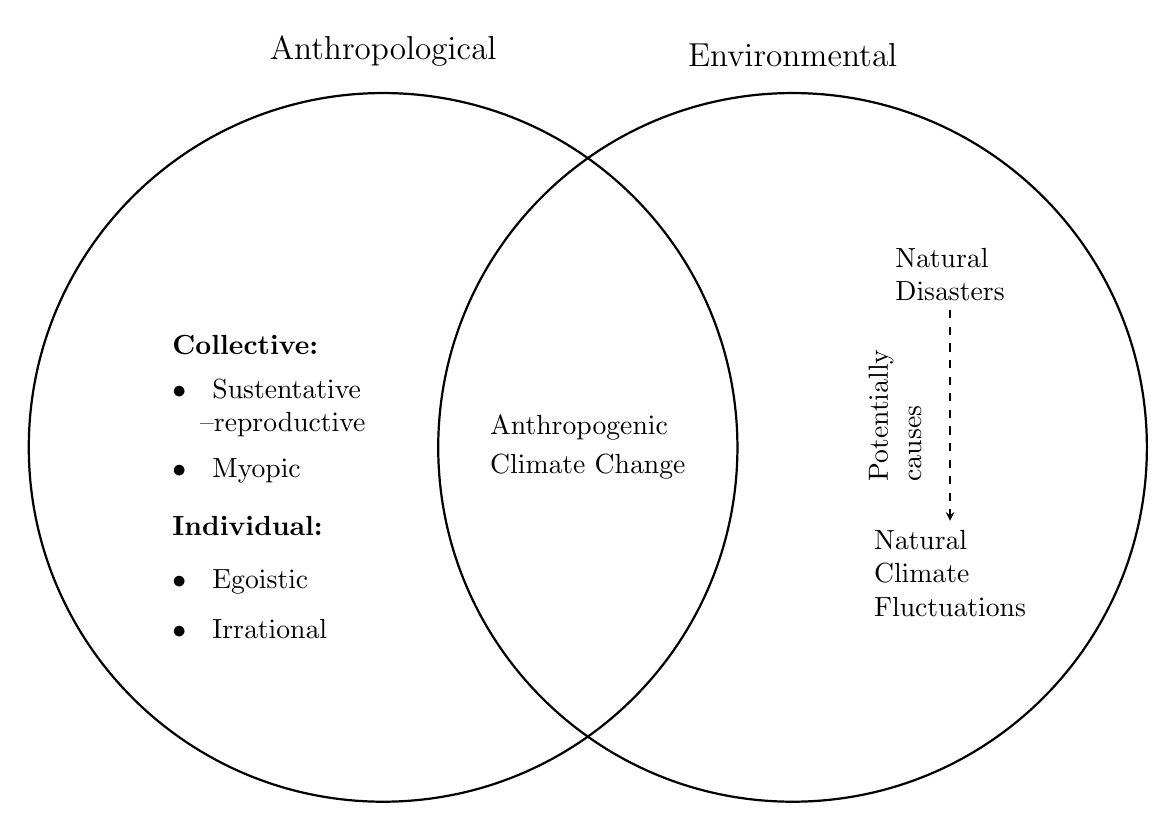
\begin{tikzpicture}[
    venn/.style={draw, thick, circle, minimum width=9cm},
    lab/.style={font=\large},
    txt/.style={align=left}
]
% Circle centers
\coordinate (L) at (0,0);
\coordinate (R) at (5.2,0); % adjust for overlap

% Circles
\node[venn] (A) at (L) {};
\node[venn] (E) at (R) {};

% Top labels
\node[lab, above=2mm of A.north] {Anthropological};
\node[lab, above=2mm of E.north] {Environmental};

% Left-circle bullet lists
\node[txt, anchor=west] at ($(A.center)+(-2.8,1.3)$) {\textbf{Collective:}};
\node[txt, anchor=west] at ($(A.center)+(-2.8,0.5)$) {$\bullet$ \; Sustentative\\\quad--reproductive};
\node[txt, anchor=west] at ($(A.center)+(-2.8,-0.3)$) {$\bullet$ \; Myopic};

\node[txt, anchor=west] at ($(A.center)+(-2.8,-1.0)$) {\textbf{Individual:}};
\node[txt, anchor=west] at ($(A.center)+(-2.8,-1.7)$) {$\bullet$ \; Egoistic};
\node[txt, anchor=west] at ($(A.center)+(-2.8,-2.3)$) {$\bullet$ \; Irrational};

% Intersection label
\node[txt] at ($(L)!0.5!(R)$) {\parbox{3.2cm}\centering
Anthropogenic\\[2pt] Climate Change};

% Right-circle text
\node[txt] (ND) at ($(R)+(2,2.2)$) {\parbox{3.6cm}\centering Natural\\ Disasters};
\node[txt] (NCF) at ($(R)+(2,-1.6)$) {\parbox{3.6cm}\centering Natural\\ Climate\\ Fluctuations};

% Dashed arrow with label
\draw[dashed, -stealth] (ND.south) -- (NCF.north);
\node[txt, rotate=90] at ($(ND.south)!0.5!(NCF.north)+(-0.7,0)$) {Potentially\\ causes};

\end{tikzpicture}
\caption{Venn diagram representing the binary theory of collapse. (Chart by author)}
\end{figure}

\newpage

\begin{figure}[h]
\centering
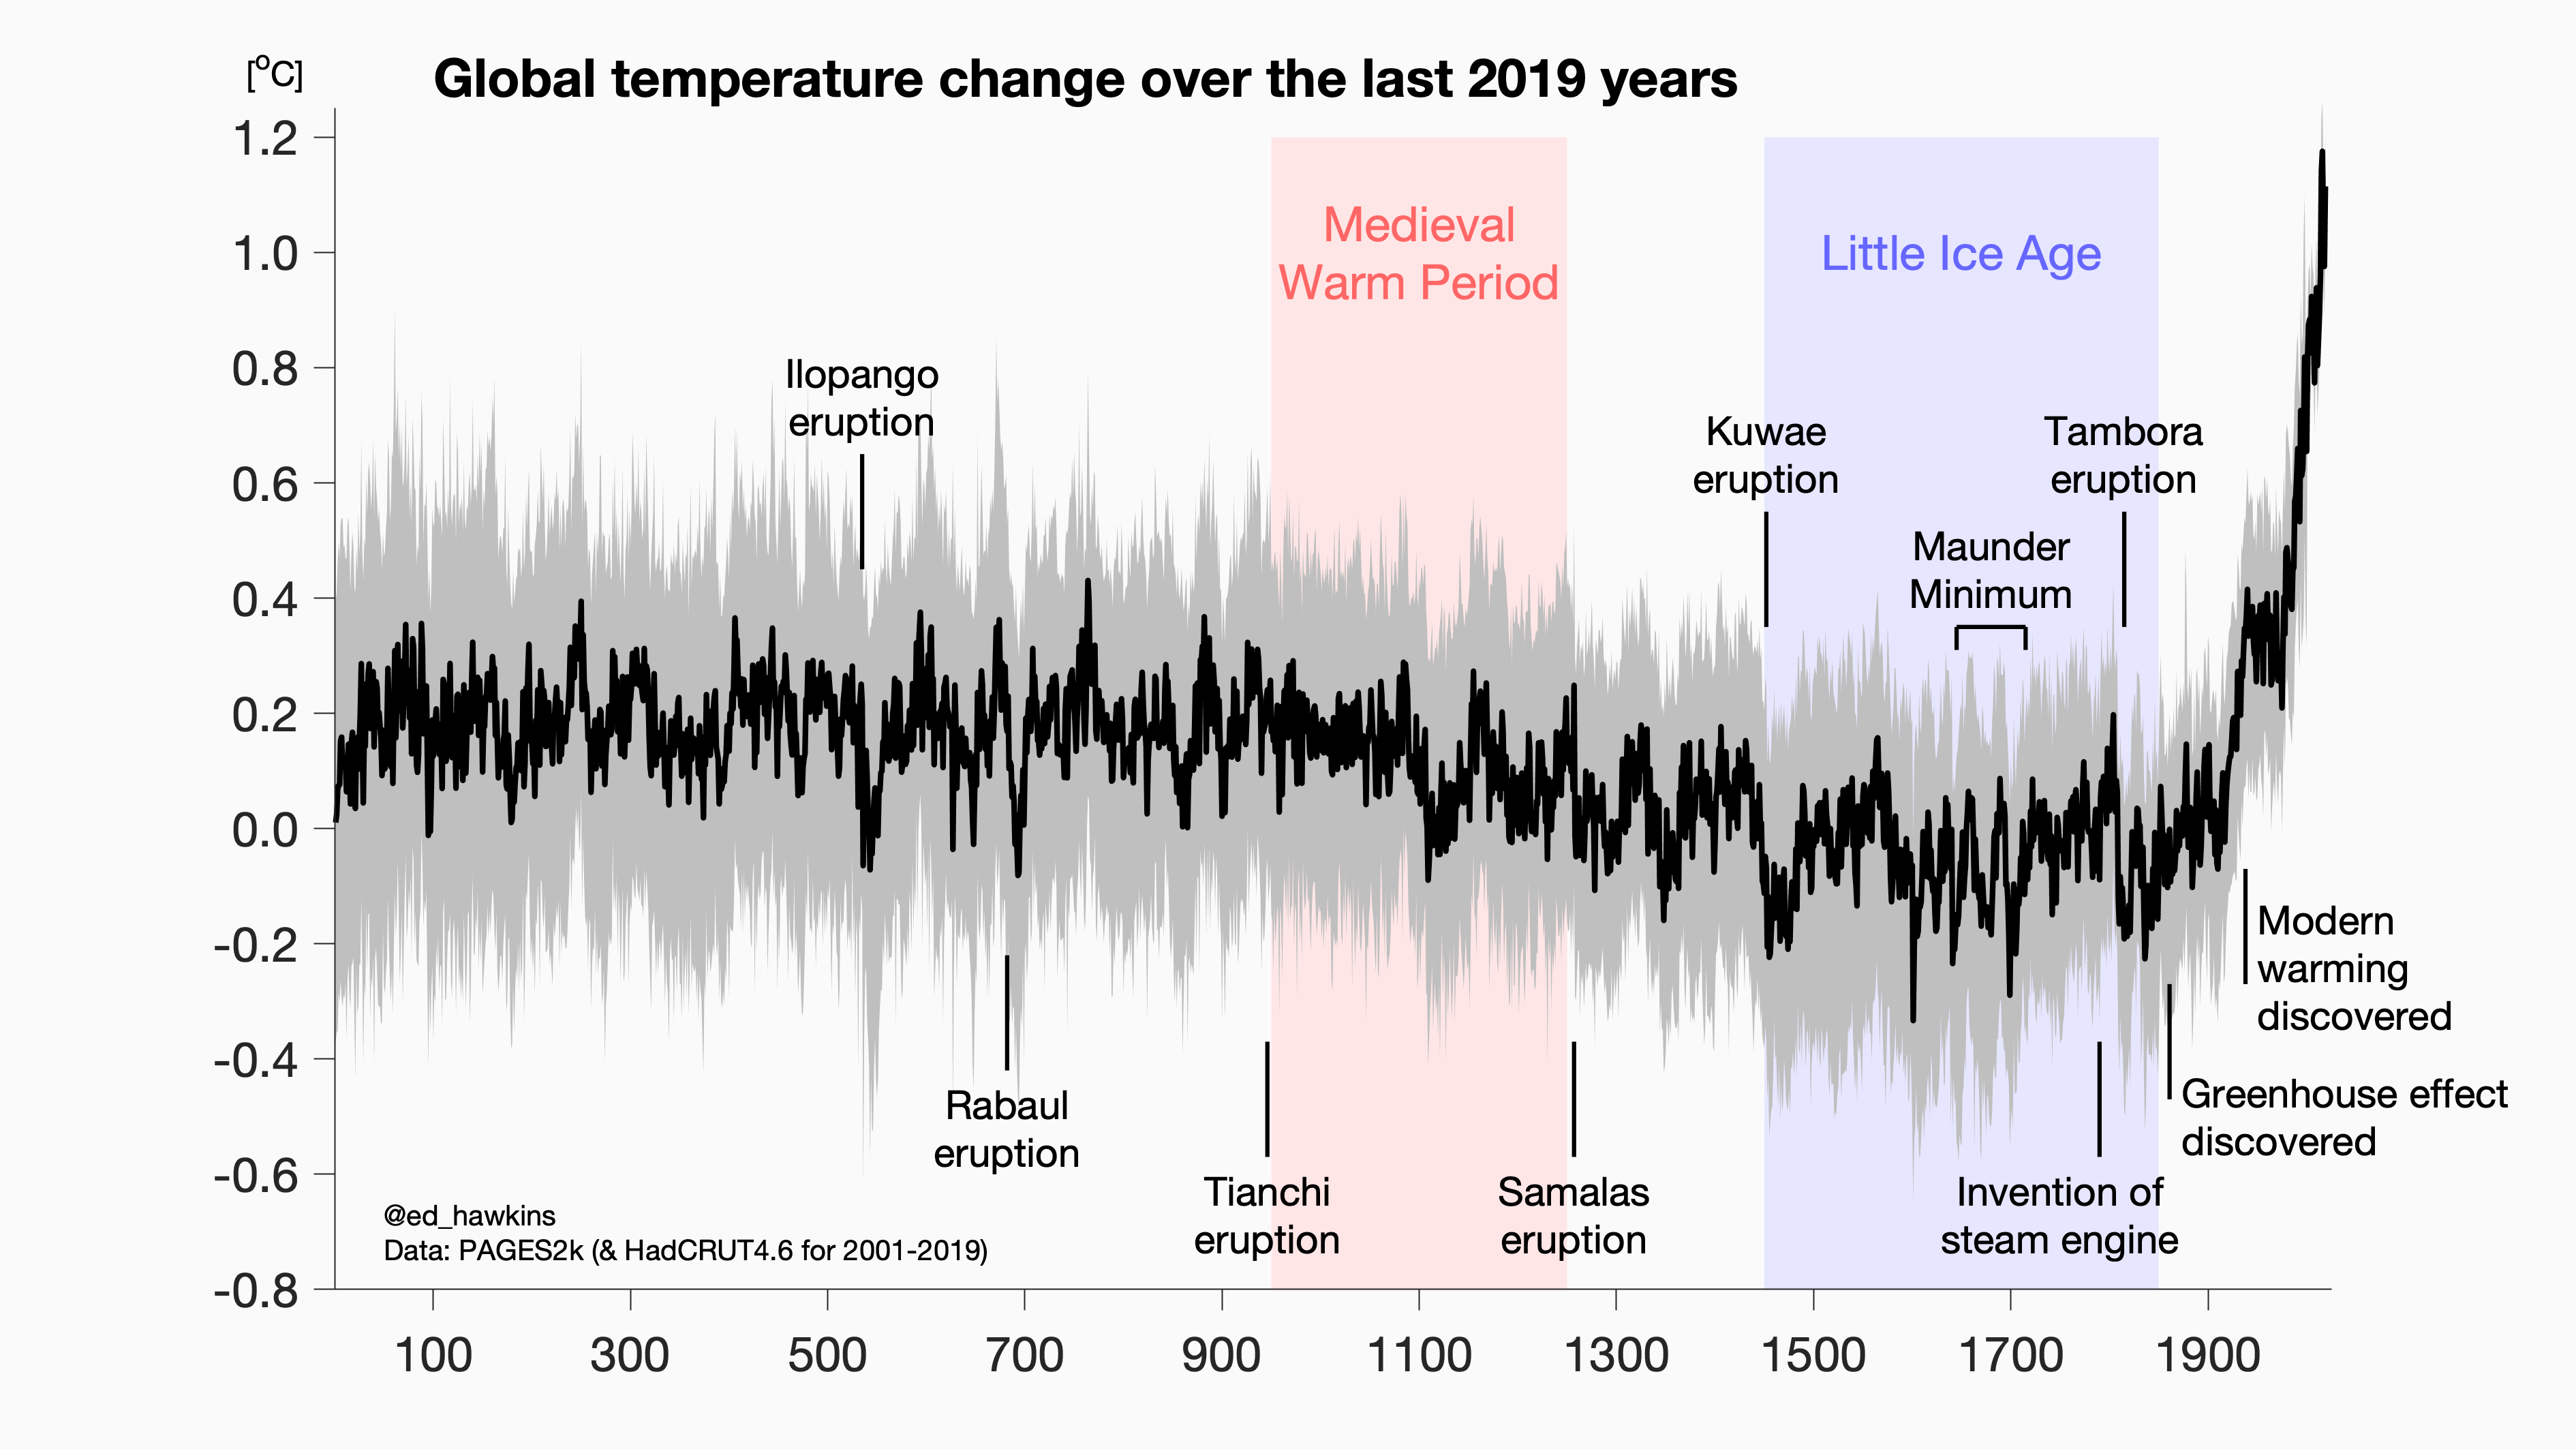
\includegraphics[width=0.9\linewidth]{lia_mwp-1.png}
\caption{The change in global temperature since 0 AD, Chart ``Global temperature change over the last 2019 years,'' from Ed Hawkin, \emph{2019 years.}}
\end{figure}

\newpage

\begin{figure}[h]
\centering
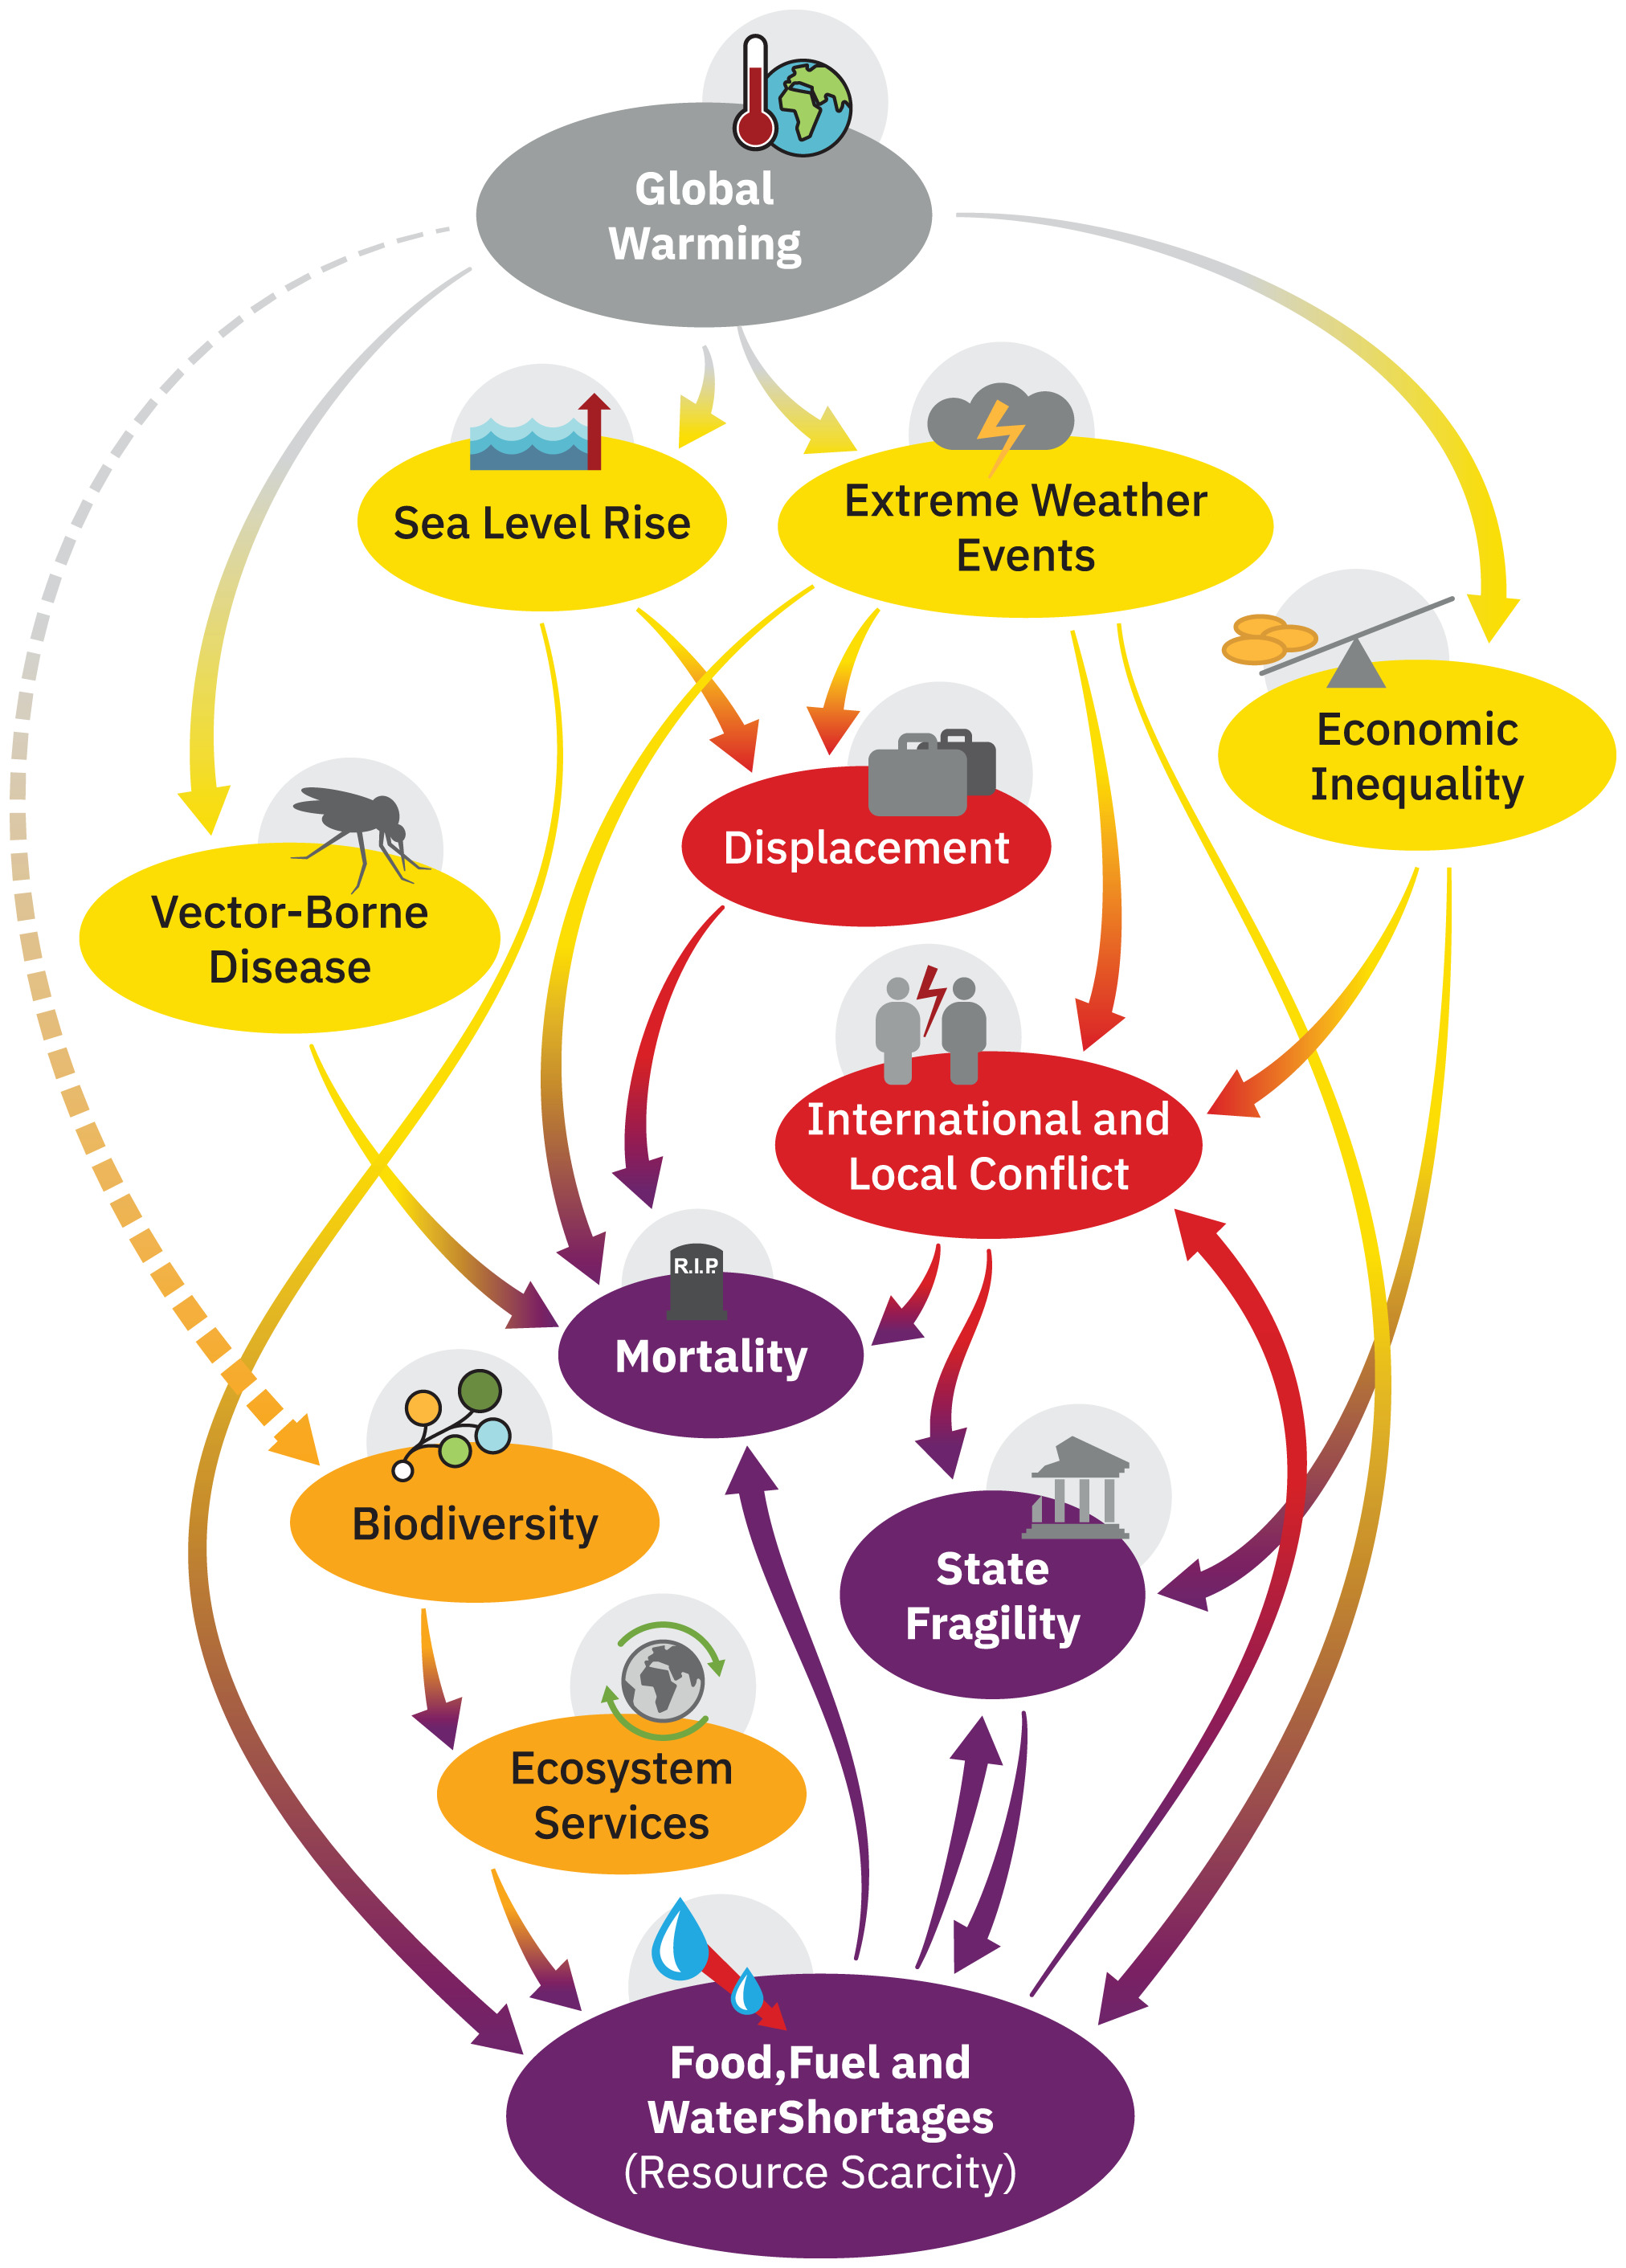
\includegraphics[width=0.6\linewidth]{pnas.2108146119fig03.jpg}
\caption{Causal loop diagram illustrating global climate failure, Chart, “Cascading global climate failure,” from Kemp et al., “Climate Endgame: Exploring catastrophic climate change scenarios”, PNAS, 119, no.34 (2022), fig. 3, \url{https://doi.org/10.1073/pnas.2108146119}}
\end{figure}

\newpage
\nocite{*}
\printbibliography[title={References}, heading=subbibliography]
\end{refsection}

\begin{refsection}[refs/evaluating]
\makechapter{Evaluating Governmental Control on Social Media Speech}{Evaluating Governmental Control on Social Media Speech}{Joseph Huang}{Acalanes High School}{10.17613/qq92m-n4548}

In recent decades, fake news—whether spread intentionally or unintentionally—has emerged as a significant challenge for countries around the world. Widespread claims of voter fraud on social media following the 2020 U.S. election undermined trust in the electoral process, resulting in reduced voter turnout in subsequent elections (Sanchez and Middlemass). Similarly, social media disinformation has fueled dangerous and violent behavior during events such as the Rohingya genocide, Southport murders, and COVID-19 (Booth; Ferreira Caceres et al.; Ortutay). Accordingly, many have argued for government regulation aimed at suppressing disinformation. However, given the practical, ethical, and economic risks of such an approach, fake news is better addressed through independent mechanisms such as third-party fact-checkers and media literacy initiatives. 

The foremost consideration when evaluating the efficacy of government regulations is their feasibility, namely, the choice of enforcement mechanisms. In Germany, the 2017 Network Enforcement Act, which relied on content removal via user complaints, prompted platforms to over‐block content, often erring on the side of deletion to avoid potential fines, while producing little reduction in disinformation (Griffin). Utilizing AI to evaluate content is likewise difficult, as AI-based takedowns yield an “enormous number of false positives”; further, algorithmic fact-checking is largely limited to English, lacking sufficient multilingual training data (Marsden et al.). Another concern is that regulation may push platforms to prioritize legal compliance over responding to evolving disinformation threats, especially as misinformation outpaces slow regulatory frameworks (Bateman and Jackson). Ultimately, the technical and structural limitations of government enforcement render it an inflexible and inefficient means of combating the spread of disinformation. 

Another concern relates to classification of misinformation: who gets to decide what “fake news” constitutes? As historical examples illustrate, especially in countries with weaker political institutions, governments have used misinformation laws to silence dissent under the guise of public safety or national unity. In Bangladesh, India, Indonesia, Malaysia, the Philippines, and Thailand, “fake news” regulation extends to government criticism; “malicious intent” clauses within such regulation justify arbitrary arrests, extended pretrial detentions, and excessive fines (Anansaringkarn and Neo; Mahapatra et al.). Singapore’s regulations allow government officials to simply declare the falsity of online information, or even the removal of said information if doing so is “deemed to be in the public interest” (“Singapore”). Often, regulation in democratic countries is used as pretext by other, illiberal states to curb press freedoms (Henley; Mahapatra et al.). Even if well-intentioned, laws enabling government regulation of social media risk centralizing undue power under state control. Thus, empowering governments to define and police fake news carries inherent risks of overreach. 

An often-neglected consideration is the effect of government regulation on the overall economy. Given that regulation increases compliance costs for platforms, the bar of entry into the social media industry rises, reducing competition and consolidating incumbent power (Sperry). The effects of government regulation on the overall economy can be illustrated by the EU’s General Data Protection Regulation (GDPR), a law designed to protect user privacy online by requiring companies obtain explicit consent for data collection and use. The GDPR serves as an effective proxy for government regulation of social media since both impose high compliance costs. As expected, following the launch of GDPR, market concentration in web tracking increased by 17\%, and websites dropped smaller third-party tracking and advertising companies who could not ensure compliance (Prasad). In addition, economic modelling indicates that repealing Section 230—the U.S. law shielding platforms from liability for user content—would eliminate roughly 425,000 American jobs, illustrating how regulation aimed at policing fake news can stifle growth and employment across an entire economy (6 Myths About Section 230). In this broader context, regulation not only undermines innovation and market competition but also imposes widespread economic costs. 

Evidently, government regulation is an inadequate solution for the issue of fake news. Combating such an issue requires an alternative approach: third-party fact-checkers. This is supported by empirical evidence favoring third-party involvement—contrasted with the lack of empirical evidence favoring government regulation. While third party fact checkers consistently produce a 10-14\% decrease in false belief and a roughly 60\% reduction in the resharing of debunked posts, rigorous studies of government regulation are scarce, most likely due to the logistical and ethical challenges of testing national laws through randomized controlled trials (Chuai et al.; Porter and Wood). Although less rigorous than randomized controlled trials and given the aforementioned challenges, public-opinion surveys offer an alternative to gauge the perceived effectiveness of regulation. One such survey conducted in Singapore indicated that only approximately 34\% of respondents reported that the 2019 Protection from Online Falsehoods and Manipulation Act stopped the creation of fake news (Ang and Zhang). This data underscores a major weakness of government regulation: not only is there a lack of rigorous evidence supporting its effectiveness, but even the sparse survey-based evidence that exists suggests it may have little real-world impact. Fact-checkers are only a temporary solution, however; a far more sustainable and preventive approach is media literacy. Although media literacy programs yield a smaller drop in belief in fake news (~0.27 SD), they produce a significant drop in the sharing of fake news (~1.1 SD) (Huang et al.). Furthermore, fact-checking requires ongoing human effort and is less effective when dealing with fake news in non-English languages, leading to higher long-term costs. In contrast, media literacy can be applied more broadly, requires fewer recurring resources, and equips individuals to assess the reliability of new information on their own (Nygren and Efimova). Together, fact-checking and media literacy provide a more effective response to fake news than government regulation. 

In essence, while the harms of fake news on social media are pressing, the challenges of enforcement, the threat of political abuse, and the suppression of competition make government regulation an ill-advised solution. Instead, independent fact-checking and scalable media literacy programs offer empirically supported, rights-preserving alternatives. The true solution lies not in restricting speech, but in equipping individuals with the tools to critically evaluate information, ensuring a more informed and resilient society. 


\nocite{*}
\printbibliography[title=References,
heading=subbibliography]
\end{refsection}

\begin{refsection}[refs/critique]
\makechapter{A Critique of the College Board Company}{A Critique of the College Board Company}{Reed Chan}{Miramonte High School}{10.17613/qq92m-n4548}

At the beginning of the twentieth century, American society saw massively expanding business and corporate consolidation in many economic sectors. Although the corporatization of industries like steel, mining, and agriculture is most popularized in American history, a very similar movement took place within the educational sector. In 1900, a group of northeastern colleges met to create the College Entrance Examination Board—the modern-day College Board—to set standardized requirements for college admissions. Although the original intent for the nonprofit was pure, to reduce the role of social inequalities in college admissions, the Board quickly took a turn towards monopolization. In the same manner that steel and oil tycoons combined resources to standardize production and dispose of competition through vertical and horizontal integration, the newly founded company wanted a standard measure to assess applicants' ability. What started as a collective attempt to corral growing applicant pools quickly turned into an educational monopoly. Throughout its lifespan, the College Board has mirrored Gilded Age corporations in privatizing and monopolizing education to maximize profits, hugely overstepping the boundaries of fair business practices today. 

Just as the Gilded Age trusts legalized and consolidated control in industry, university managers pursued standardization as a shield against unmanageable admissions. As enrollments grew and candidates differed in background and preparation, one objective examination appeared to impose order, meritocracy, and efficiency–the SAT. Beginning as early as 1926, the proposed standardized test promised to eliminate bias from college admissions by testing each student on equal grounds. Such efficiency, however, had unintended effects: secondary schools, always responsive to college entrance demands, adapted curricula to College Board designs. This undermining of the corporation's initial goals not only created a "teach to the test" style of high school teaching but also encouraged further dependency on the College Board by schools across the nation, as universities began to accept the SAT as a standardized test. The rise of the SAT catapulted the College Board corporation into becoming an industry leader, with the corporation’s reported 2019 revenue being over \$1.1 billion (\cite{totalregistration}). But how has this seemingly “nonprofit” organization gained this much revenue? Well, standard SAT and AP test fees can easily add up to over \$100 per test. Since these tests are essentially mandatory for millions of students nationwide, the College Board profits massively. Not only this, but the College Board also profits from illegally selling student data. In 2024, the College Board was caught sharing and selling student data in violation of New York State’s student privacy law (\cite{desantis2024}). Eventually receiving a \$750,000 penalty, the College Board continues to illegally profit off of unaware consumers. In true robber-baron fashion, the CEO of College Board, David Coleman, earned over \$1.6 million–all while exploiting and mercilessly upcharging his customers. By tracing the College Board's ascent, we can discern a broader trend: the privatization and corporatization of public spheres once thought inviolate to market influences. The Board's transformation from modest exam administrator to corporate overlord of educational access reflects the twentieth century's broader Gilded Age movement towards cold, privatized, profit-driven monstrosities that control our futures.

The abominable nature of the corporation has sparked extreme debates over the company’s legitimacy. Authors like Richard P. Phelps contend that the organization's control over standardized testing is a mirror image of the monopolistic behavior of its Gilded Age forebears, employing its market dominance to suppress competition and increase clout (\cite{phelps2018}). With this in mind, the Sherman Antitrust Act–originally crafted to dismantle Gilded Age monopolies–offers a potential legal avenue to challenge the College Board’s dominance. The corporation’s complete control over college admissions testing and curriculum could be viewed as unlawful monopolization, warranting full federal intervention. In a recent editorial in the California Law Review titled “The College Board: A Case for Antitrust Enforcement Under Section 2 of the Sherman Act”, it is noted that the Board's monopoly on admission examinations provokes valid antitrust issues due to the absence of acceptable alternatives, increasing its monopoly power (\cite{kronsburg2025}). Ultimately, the College Board is a perfect representation of Gilded Age corporate abuse of power, only in our own society today. Similar to famed policy-makers like President Taft and heroic muckrakers like Ida Tarbell, we must fight these tyrannical corporations for the betterment of students across the nation.

The best way to combat such abuses, at least for a student like me, is to raise awareness against these injustices. The Fabric of a Nation Textbook effectively covers the relationship between industry, labor, and political reform of the Gilded Age, but does not include how such corporations have continued into the current age, especially in less mainstream industries like education. A necessary change to the APUSH curriculum to better inform students of the current day could be to add specific examples of late 19th-century corporations that still exist today (like College Board, itself), and further explain the limitations and failures of policies made to hinder such corporations. Overall, the College Board's transformation—from a club of elite colleges to a centralized testing behemoth—mirrors the consolidation of economic power during the Gilded Age. Its influence on curricula and college admissions illustrates the trade-off between public good and privatization, and equity and efficiency. As students learn about the legacy of the Gilded Age, we must garner a more complex understanding of both the period that gave rise to it, but also how its themes persist to the current day.


\nocite{*}
\printbibliography[title=References, heading=subbibliography]
\end{refsection}

\begin{refsection}[refs/fertility]
\makechapter{A Fertility Crisis}{A Fertility Crisis}{Justin Lee}{Oakland High School}

\begin{abstract}
As of 2017, half of the world population resides in a nation with a below replacement level population structure (\cite{frejka2017half}). By 2100, however, 97\% of the world will have a fertility below that of the replacement rate – leaving only six nations able to grow or sustain their population (\cite{thelancet2024dramatic}). Needless to say, declining fertility rates are a hugely existential and complex, if not highly urgent problem. This essay, then, will seek to only briefly investigate the fertility crisis by outlining its causes and repercussions and arguing for what I believe to be the most promising solution. 
\end{abstract}

Roughly, there are three categories of causes which have led to a fertility crisis: socio-cultural, economic, and biological.  

Socio-cultural factors include secularization, urbanization and an increasing focus on the quality rather than quantity of children. According to a poll by Gallup, people are as non-religious as they have ever been, from 0\% of people identifying as non-religious in 1954 to 21\% in 2022 (\cite{newport2022slowdown}). Then, as religiosity is linked to fertility, this trend has no doubt contributed to a decline in the fertility rate (\cite[p.\ 85]{kearney2023causes}). Urbanization also plays an important role in reducing fertility rates, as when families move into cities, a demand for manual labor, present in the countryside, but  disappears, eliminating a key incentive for parents to have more children (\cite{bricker2021birthrates}). Also, a cultural shift towards having less, rather than more, higher quality has tempered parents’ desire for multiple children (\cite[p.\ 84]{kearney2023causes}).  

Economic factors mainly describe factors general fears regarding the economy, such as fears of job insecurity and the increasing costs of raising children. An excellent example of financial uncertainty causing a decline in fertility is during recessions, as amid such events, fertility rates have consistently fallen (see Figure 2) (\cite[p.\ 83]{kearney2023causes}). Moreover, when families are burdened by debt or when they have little disposable income, they are less likely to have children (\cite[pp.\ 82, 84]{kearney2023causes}). Exacerbating this problem is the rising costs of raising children; in the last decade alone, the cost of childcare had risen by 28\% (\cite{usafacts2022childcare}). As these trends persist, demand for children will continue to slump (\cites{becker1960economic}{lino2017cost}). 

Biological factors relate to the development of contraceptive technology, rising infertility, and reliance on fertility technology such as in vitro fertilization (IVF). In recent decades, contraceptive technologies have increasingly been made available. In fact, from 1955 to 1965, an estimated 40\% of the reduction in fertility rate was facilitated by access to contraception (\cite[p.\ 25]{bailey2010mommas}). Furthermore, studies have shown that biological factors such as poor semen quality, infertility, and increasing rates of testicular cancer caused by environmental pollution have also contributed to a decline in fertility (\cite{skakkebaek2022environmental}).  

Having discussed the causes of the crisis, we can now proceed with discussion of its ramifications. The main consequence of a depressed fertility rate is its macroeconomic effect, as the size of the economy (or GDP) is dependent on the size of its workforce, as well as on the number of pensioners. According to the Solow Growth Model, GDP is directly proportional to workforce size; therefore, if the size of the workforce were to be reduced, then the economy would similarly contract (\cite{solow1956contribution}). Although \emph{ceteris paribus}, per capita GDP would remain constant while the workforce shrinks, a diminished GDP means that overall spending on public goods may decrease, resulting in a tighter defense or education budget (\cite[p.\ 88]{kearney2023causes}). Aside from this, the dependency ratio is also a key factor affected by falling fertility rates. With less working age population and more pensioners, the government must spend more in terms of social benefits and/or the children of the elderly must have greater support for their parents financially, both of which puts strain on the economy (\cite[pp.\ 91–92]{kearney2023causes}). Lastly, inflationary pressure and curtailed innovation have also been proposed as consequences of the fertility crisis (\cites{jones2022end}[p.\ 18]{kohler2006low}).

Despite these detractions, however, there are perks to low fertility. Under such circumstances, the cost of equipping new workers would fall, environmental pressures would ease, and the impact of an increasing skewed dependency ratio is projected to be counterbalanced by increased investment in human capital, hence improving the efficiency of workers (\cites[p.\ 3]{jarzebski2021ageing}{lee2010fertility}[p.\ 7]{lee2014low}). An additional consideration lies in the increasing automation of many industries, such that demand for human labor may decrease in the future. However, in spite of presently addressed concerns, a normative argument could still be made, as by attempting to raise fertility rate, there are only minor drawbacks, while the potential for catastrophic consequences if fertility is left unchecked are immense. 

When considering potential remedies to the fertility crisis, perhaps the most conspicuous solution is pro-natal governmental suasion. Such examples include financial incentives, expanded employment benefits, subsidized childcare, and housing subsidies. Propagandizing efforts to change social perceptions of children may also be adopted through art (see Figure 1), slogans, and other media (\cite[p.\ 37]{kohler2006low}). Indeed, this is the method adopted by many nations around the world today.

For an example, we can turn to Singapore, which began to introduce explicitly pro-natal policies beginning in 2001. Singapore initiated policies to make working environments more accessible for those wishing to start a family, subsidized reproductive technologies like IVFs and contraception, and offered low-cost, high-quality formal childcare. These comprehensive measures, however, achieved only limited success, failing to produce long-term, concrete results (\cite{tan2020lessons}).

Rather than direct governmental interference, I argue that the most effective method of combating low fertility rate around the world is through the continued focus on implementation of policies which strengthen and stabilize the overall economy, while adopting a “homeostatic” stance towards population. Through focusing on fundamental issues such as reducing unemployment, promoting free international trade, fostering innovation and other such matters, we absolve people’s insecurities regarding their and their potential children’s future. This mitigates a central motivation in the reduction of fertility, while avoiding superfluous governmental interference. Compared to the interventionist approach, where there exists only a weak correlation between implemented policies and increases in fertility, focusing on improving future economic outlook has historically been an effective promoter of economic stability (\cites[pp.\ 93–97]{kearney2023causes}{stern2022ways}). Additionally, the Easterlin hypothesis states that as labor supply falls and demand rises, wages also grow, generating demand for children and inducing a rebound in fertility (\cites{easterlin1987birth}[p.\ 31]{kohler2006low}). Though such a stance towards population planning is currently theoretical, it seems the most cost-effective and laissez faire solution to the fertility crisis, letting population dynamics simply be influenced by organic economic forces. 

\newpage

\begin{figure}[h]
\centering
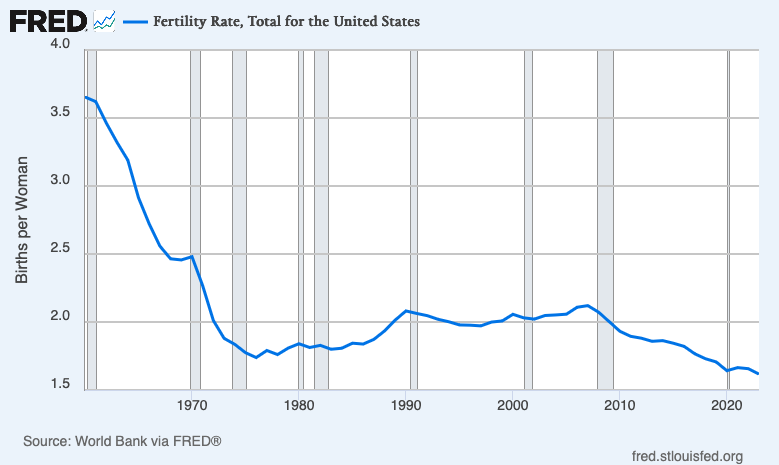
\includegraphics[width=0.6\linewidth]{fredgraph.png}
\caption{US fertility rate trend 1960–2022, overlayed with US recessions. From \emph{Fertility Rate, Total for the United States}, by World Bank, 2024. (\url{https://fred.stlouisfed/series/SPDYNTFRTINUSA}). Copyright 2024 by the Federal Reserve Bank of St.\ Louis.}
\label{fig:1}
\end{figure}

\begin{figure}[h]
\centering
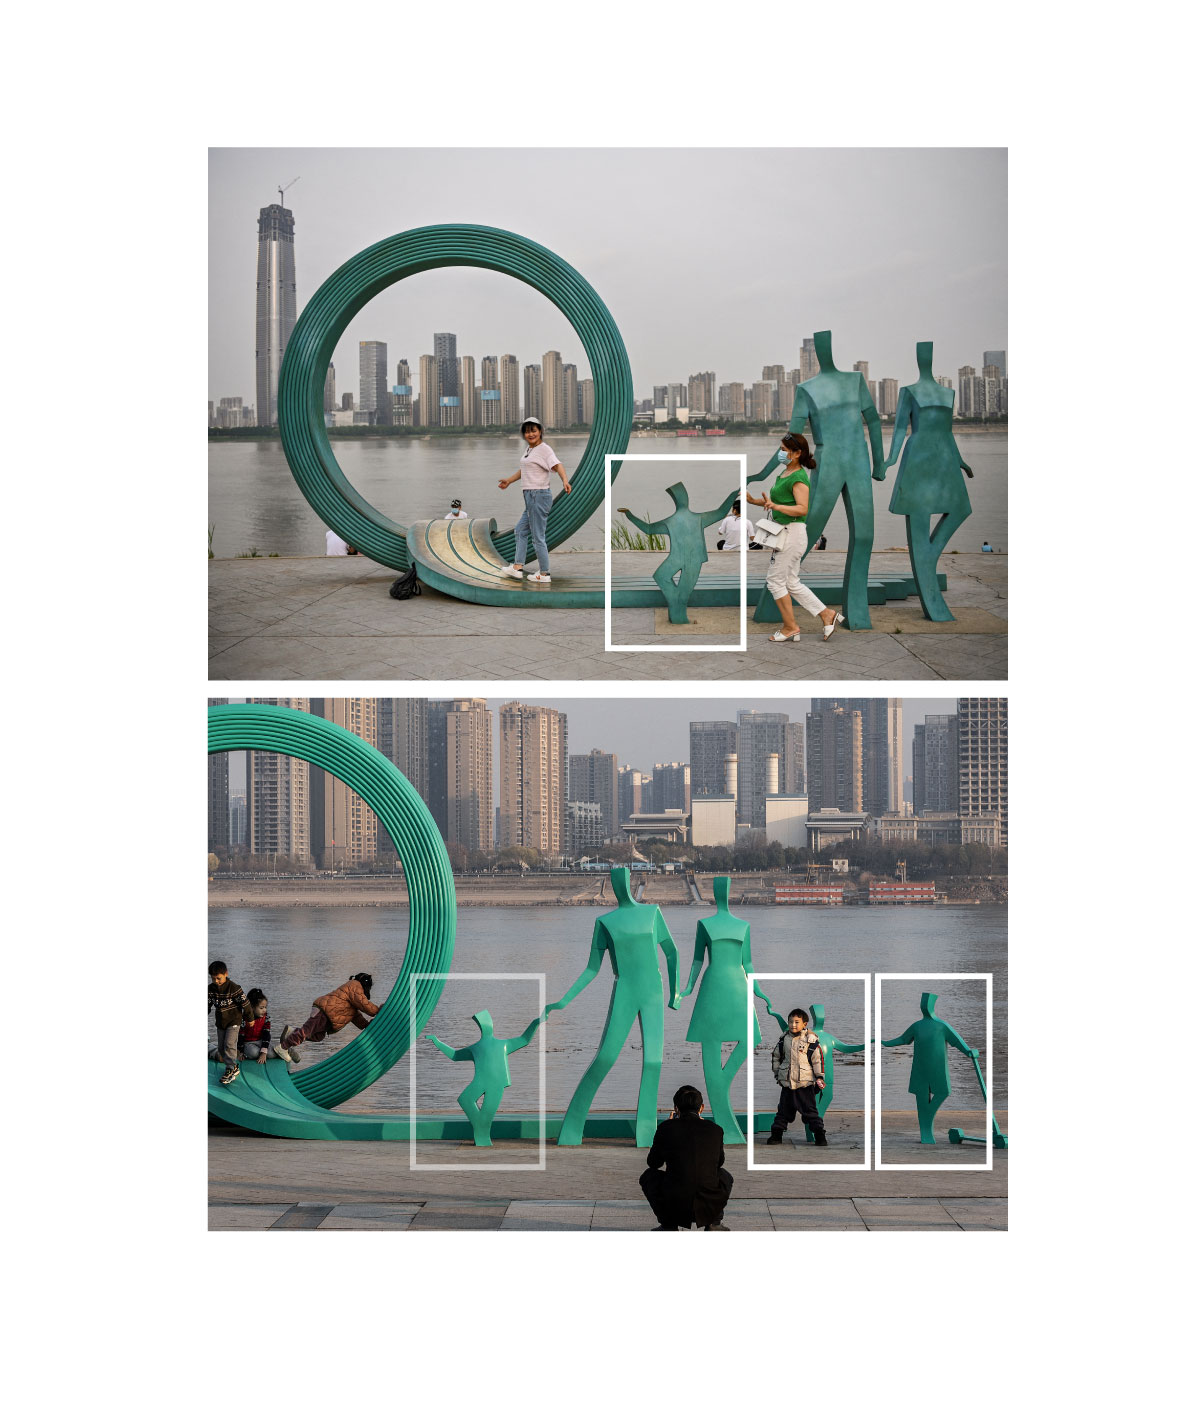
\includegraphics[width=0.5\linewidth]{top-600.jpg}
\caption{A sculpture in Wuhan, a city in central China, depicted a joyful family of three. Recently, two more children were added. From \emph{Three Is Best: How China’s Family Planning Propaganda Has Changed}, by Isabelle Qian and Pablo Robles, 2024. (\url{https://www.nytimes.com/interactive/2024/03/09/world/asia/china-childbirth-propaganda.html}). Copyright 2024 by The New York Times Company}
\label{fig:2}
\end{figure}

\newpage


\nocite{*}
\printbibliography[title=References,heading=subbibliography]
\end{refsection}

\begin{refsection}[refs/racism]
\makechapter{A History of Racism and a Case for Affirmative Action}{A History of Racism and a Case for Affirmative Action}{Michael Gkatzimas}{Miramonte High School}

Racism is an intrinsic flaw in our society that echoes across our institutions, economic and class hierarchy, and current global political formation. Racism continues to be an issue today due to its deep-rooted importance in the creation of our society and the status quo. In order to begin fixing such a fundamental piece of our society, we must first define racism itself, examine its origins in early European colonialism, its eventual systematic oppression of minority groups, and finally, discuss the benefits and flaws of affirmative action - a proposed solution to the complex topic problem of racism. Although not perfect, affirmative action, grounded in the ethical theories of utilitarianism and Kantianism, is an effective and morally correct approach to addressing the historical and ongoing impacts of interpersonal and systemic racism.

To understand the topic of racism, we must first determine what race is. Contrary to popular belief, race was originally used as a method of organization based on class rather than physical features. The modern definition of race, however, is a societal construct originally designed in the 17th century in Western Europe, created to classify people into “natural groupings” based on physical features and observed behavior. This concept was created by Swedish botanist Carolus Linnaeus and German physiologist Johann Friedrich Blumenbach, who applied the concept of the “natural” hierarchy of various flora and fauna to groupings of people (\cite{smedley2024}). Although not initially malevolent, this divisionary concept of race quickly gained attention, as many Enlightenment thinkers and writers in Western Europe began to support this idea. Many assertions about the inferiority of specific races (typically targeting Africans) were published. Notable philosophers and thinkers such as Voltaire, David Hume, Thomas Jefferson, and Immanuel Kant all expressed negative opinions about the “primitive” nature of Africans. This trend of superiority saw its peak with the rise of Social Darwinism, a misnomer that twisted Charles Darwin’s biological theory of evolution (survival of the fittest) and applied it to race. This theory was created by Spencer and Walter Bagehot, who used it as a “scientific” way to further categorize races. This form of racism, now defined as discrimination or prejudice based on racial or ethnic groups played a major role in shaping the formation of our society today. Although many motivations existed for the rise of colonial movements in Europe, including the desire for economic gain, political advantage, and the spread of religion, one of the most intrinsic motivations that allowed colonists to commit such acts of extreme violence and exploitation was the self-righteous belief that the white man was key to civilizing a society. Spurred on by ideas of European superiority and perfection, colonial settlements across Africa, the Americas, and East Asia saw extreme exploitation of the native population. Social disruption, proselytism, mass killings, and forced labor were only a few of the appalling ramifications of early imperialism that were justified by the idea that European colonists were civilizing the savage and barbaric non-European population and bringing them the light of religion and “proper society” (\cite{kipling1899}).

Now that we have generally established the definition of racism and its origin, we must break down the specific subcategories of racism, their prominence in history, and their permanence today. The complex issue of racism can be broken down into two separate subcategories: interpersonal racism and systemic racism. Interpersonal racism is the most general form of racism, where conscious or subconscious bias plays a role in influencing interactions or perceptions of other people based on race. This form of racism is most often expressed in stereotypes and racial slurs, as well as in more violent forms such as hate crimes. Typically influenced by social norms, a historical example of interpersonal racism is the brutal conditions under which Africans were kidnapped and transported to the Americas in the system known as the Trans-Atlantic Slave Trade. In this system, goods and cash crops obtained through slavery in America were traded for African slaves captured across coastal regions of Western Africa. Infamously, the Middle Passage (transportation of slaves from Africa to the Americas) was known for its extremely overcrowded and destitute living conditions. Facing disease, malnutrition, and physical and mental abuse, around 12.5 million Africans, primarily males, were enslaved and taken away from their homes to work on plantations until their deaths. Interpersonal racism played a large role in the slave trade due to evolutionary beliefs in Social Darwinism, Africans were viewed as closer to creatures than humans. This dehumanization of a targeted race has been a common theme throughout history, with such forms of racism still relevant to us today. 

Interpersonal racism in the form of hate crimes has seen a massive increase in recent years, with almost 12,000 hate crimes being committed in 2022, compared to 7,200 in 2018. More specifically, violence against Asian Americans has seen a marked rise following the COVID-19 pandemic. The virus’ Chinese origin caused many people to associate Asian Americans with the virus, leading to the increased use of racist remarks, stereotyping, and violence. From the start of the pandemic in 2019 to 2020, the FBI reported a 77\% increase in hate crimes against first- and second-generation Asian Americans (\cite{findling2022}). Hate crimes make up only a small percentage of interpersonal racism. The most common forms are verbal abuse and discrimination. A study done by the American Journal of Public Health found that calling COVID-19 the “China Virus,” a label given by former President Donald Trump, was heavily associated with more frequent instances of bias and hate speech against Asian Americans (\cite{hswen2021}). This further illustrates how interpersonal racism follows societal trends created or endorsed by influential figures and continues to target and attack specific racial minorities. 

Now, let's discuss the topic of systemic racism, the form of racism that has been most influential throughout history and today. Systemic racism is defined as policies and practices that exist throughout society that result in discrimination or biased, harmful treatment of others based on race. Examples of systemic racism throughout US history include the Chinese Exclusion Act of 1882, which was the first legislation to ban immigration targeting a specific racial group. This act was preceded by extremely high racial tensions, where the increasing Chinese immigrant population was blamed for unemployment and low wages. This blaming of Chinese immigrants, known as scapegoating, is a common motivation for systemically racist policies. Similarly, during World War II, the American public feared that Japanese American citizens were spies for the Japanese government. They were forced into government facilities known as internment camps. Signed off by President Franklin D. Roosevelt, armed military personnel forcefully removed Japanese Americans from their homes and transported them into internment camps across the country. Lasting for over three years, these camps had terrible living conditions, with almost 2,000 Japanese dying in these camps due to a lack of medical care. After the war ended, thousands of Japanese were displaced, without homes and jobs. Japanese internment remains one of the worst instances of institutionalized racism in America’s history; this illustrates the deep-rooted racism that is built into this country. One of the biggest institutions of systemic racism in American history by far, however, was the use of Jim Crow laws in the South. Enacted in the late 19th century, Jim Crow laws racially segregated almost all aspects of life (schools, restaurants, public places, transportation, etc.). These policies were created to continually oppress African Americans and to perpetuate the status quo of white supremacy following the abolition of slavery. During this time, blacks faced policies such as “redlining” - policies that isolated black communities into poverty and instituted a cycle of crime, over-policing, and poverty that we still see today. Racial profiling and police brutality reinforce this system of oppression. Because of the stereotype of blacks being criminals (perpetuated by low wages leading to increasing crime and policing in black neighborhoods), around 41\% of African Americans report being stopped by a police officer solely because of their race (\cite{stewart2024}). Not only this, but blacks face a disproportionately high rate of police brutality, with 25\% of all people killed by law enforcement being black males (black males comprise only 6\% of the population). Institutionally racist policies of redlining, the biased criminal justice system, racial profiling, and police brutality all contribute to a cycle of racism, poverty, and a lack of effective change that only perpetuates the corrupt status quo of today.

While no solution will perfectly end all forms of racism, affirmative action remains the best option for combating and ending the deep-rooted cycle of racism that our country was built on. Affirmative action is defined as a set of policies that seek to benefit marginalized groups, working to bridge inequalities in pay, education, and employment. Forms of affirmative action can be categorized into three categories: outreach (offering marginalized groups opportunities), remedial (offering compensation to historically disadvantaged groups), and diversifying legislation. Examples of such policies include introducing quota systems, meaning organizations are required to give a certain number of positions to disadvantaged groups. Initially created in an attempt to end discrimination in the 1960s, quota systems attempt to end inequities in employment, education admissions, roles in politics, and others by diversifying the workforce and ensuring that all people have an equal chance at success regardless of the opportunity given from birth. Many quota systems have seen success in employment - a study conducted by the United Nations University in Europe found that 63\% of the 194 studies reviewed concluded that affirmative action improved “outcomes for ethnic, religious, or racial minorities“ (Gisselquist). Affirmative action has not seen universal approval; many universities in the US have recently pushed back on diversity quotas in admissions, arguing that affirmative action removes the core meritocratic nature of admissions. On June 29, 2023, the Supreme Court ruled that using race to determine college admissions is ultimately unconstitutional, sentiments supported by the banning of affirmative action in public colleges across nine different states. The amount of discourse around affirmative action brings the policy’s morality into question. In order to analyze such a contentious topic, let’s analyze affirmative action through the lens of utilitarianism and Kantism. 

The principle of utilitarianism deems that an action is considered morally correct if it promotes the greatest happiness for the greatest number. When analyzing affirmative action under Act Utilitarianism (a branch of utilitarianism prioritizing short-term happiness for a specific act), policies such as quota systems may seem immoral, as such policies may have the opposite effect of increasing racial tensions between minority groups, possibly leading to “reverse discrimination” (often called anti-white racism) and increasing hate crimes and acts of racism, rather than increasing success and equality. Under the lens of Rule Utilitarianism (a branch of utilitarianism that conforms to determined laws or rules, typically favoring long-term gain), however, affirmative action is much more appealing, as quota policies ultimately increase diversity in the workplace, leading to more overall success and happiness across racial groups, as well as mending the damage of oppressive systematic racism.

In Kant’s deontology, an action is defined as morally correct if it can be universalized without contradiction, respects other humans as an end (all humans autonomously reason) rather than a means, and is purely driven by duty rather than consequence. Affirmative action can be applied universally without contradiction, as the primary goal of such policies is to introduce equity and balance the inequalities of birth-given opportunities (something that will always be true regardless of universality). Those who argue against affirmative action often cite the rise of tokenism and ineffective policy as negative consequences of affirmative action. Tokenism, or the practice of meeting diversity quota requirements solely to give the appearance of diversity, is treating other humans as means rather than an end (treating someone as a diversity check box rather than a human being). Nonetheless, affirmative action is morally correct as the basis of such policies appeals to the duty to uphold the basic principle of equality (that differential treatment is justified in morally different situations) rather than achieving peak efficiency in the workforce or other consequentialist concerns.

Overall, affirmative action is a flawed yet effective way of ending the cycles of racism and poverty that have been perpetuated throughout our country's history of systematic and interpersonal racism. While issues such as tokenism and ineffective policies exist, the goal of affirmative action is to lead society toward a healthier and more equitable future. Meritocratic systems must be rewritten to account for differing opportunities, something that is only solved through affirmative action policies such as reimbursement of disenfranchised communities and diversity quotas. “Reverse discrimination” and rising tension between racial groups may be a consequence of diversity, but it is a necessary part of transforming our broken society into one of true equality and opportunity. While there will always be those disadvantaged by affirmative action policies, those experiencing the benefits (marginalized communities) deserve their own equal opportunity after being subjected to decades of systematic oppression. 



\nocite{*}
\printbibliography[title=References,heading=subbibliography]
\end{refsection}

\begin{refsection}[refs/china]
\makechapter{China's Lost Children}{China's Lost Children, its Dying Economy, and the Economic Implications}{Kevin Nguyen}{California High School}{10.17613/8rcyg-n5q57}

First implemented beginning 1980, the One Child Policy (OCP) was a policy formulated by the Chinese Communist Party (CCP) with the goal of reducing the birth rates in a quickly industrializing China. By reducing population growth, the government hoped to avoid a Malthusian catastrophe and maintain an “optimal” population for China (L.\ Jiang) Throughout the existence of the policy, it saw a general trend in the gradual loosening of enforcement and growing number of exceptions to the policy. Despite this, the policy still managed to cause an enormous impact upon population demographics, preventing the birth of 100 to 400 million children (Q.\ Jiang), and radically skewing the gender ratio (Brittanica), causing an estimate of 3-4\% more males than females in China. Part of the consideration during the inception of the policy was that the OCP would allow for an increase in the ratio of working age adults to children, which would incentivize saving and increase productivity. While this was the case in the short term, in the long term (Feng), the OCP would cause a shrinkage and expansion (Silver \& Huang) of the working age population and the elderly population respectively, augmenting the strain upon welfare programs and taxpayers. These varieties of factors would not only have a profound effect on the Chinese economy, but consequentially, on the international economy. 

There were some benefits that came with the OCP. Mainly, lowering the fertility rate can result in demographic dividends (International Monetary Fund) that spur economic growth, a result of the diminished dependency rate (i.e., the ratio of the working populace to the non-working populace). Savings rates also increased by 7.5\% (Q. Liang), contributing 25\% to the growth of the Chinese economy, though this disputed, with some sources stating that the contribution of the OCP to saving rates is negligible (Song). The OCP was advantageous in other ways as well, increasing output per capita, narrowing the wealth and gap, and decreasing skill premium (Liao). However, there were also downsides presented by the OCP.  Families with more than one child spend more (Keyu), thus contributing to the economy. Often, this spending goes into education for the child, which serves to further the economic development in the future. The rise in dependency rates as a result of a rise in the proportion of the elderly population and legal obligation of China’s youth to support its elder will cause a contraction of the economy (Mansharamani). Unlike other Asian countries facing the same problems of a declining population of the working age, China has one of the highest female labor-participation rates in the world, being 60.5\% in 2023 (World Bank). This means that the potential effects for increasing female participation in labor is limited. According to some estimates, by 2035, 32.7\% of the population is expected to be 60+ (Economist Intelligence), 60 being the retirement age for males in China, females being even lower. As a result of the skewed gender ratios, men in China used the ownership of property as a sign of affluence, causing the formation of a housing crisis as men rush to purchase property and caused an oversaturation of the housing market. Construction has fallen by 60\% relative to pre-COVID levels (Hoyle), seriously impacting the Chinese economy. Further compounding the problem is the lingering cultural impact of the OCP, as the current generation does not want more children (Stanway), exasperating labor problems in the Chinese economy for the future. 

First, the shrinkage of the working age population in China is beginning to cause, its imports and exports will also begin to weaken, impacting the global economy. Just last month, China’s exports and imports declined by 7.5\% and 1.9\% respectively (Soo). Last year, China’s imports dropped by a little less than 9\%. This recent change reflects a growing trend of falling exports and imports, which can grow to have a profound effect on the global economy (Marsh). Companies such as Apple, Volkswagen, and Burberry rely heavily upon the consumer market in China (Marsh), had begun and will continually be impacted by the atrophying Chinese economy. There is evidence that in addition to the OCP, the apparent economic downturn wMarshas a result of the trade war between the United States and China, which has led to dramatically reductions in trade between the two countries (Bown).  

Second, the massive increase of saving rate, rising 20\% from 1983 to 2011 (Coeurdacier), was a result of many factors including low amounts of urbanization, lack of a social safety net, the strong growth rate of the economy, and the OCP (Hung). The result of this is that the money, instead of going back into the economy as money spent by consumers, instead wound up in peoples savings accounts. A high saving rate causes a litany of problems, including increased pressure on interest rates, causing excess investments, and leading to decreases in exchange rates (Song). A more balanced gender ratio may resolve this issue (Wei), and furthermore, reduce tensions between China and its trading partners.  

Third, the aforementioned gender imbalance brought about by the OCP in China has also caused a housing crisis, effecting the global housing market in the process. China is experiencing a decline in the demand for steel, cement, glass, etc. (Nunley), which is detrimental to the export economy of other nations. In addition to this, as a result of property owners’ unwillingness to sell their property at low rates, commercial property deals have sunk to record low levels globally (Real Estate Markets to Be Invigorated as Growing Pool of Buyers and Sellers Look to Make
a Splash.). Chinese investors who had invested aggressively in decades past have mostly resorted to off-loading projects in the face of the housing crisis (Callanan). In China, the fact that real-estate contributes to 22\% of the total GDP, combined with the fact that a drop of ~4.25\% in the Chinese GDP would cause a ~1.5\% drop in the GDP of advanced economies and a ~2.75\% drop in the GDP of emerging economies certainly makes the situation seem grim (Rogoff). 

The effects of the OCP, despite being highly controversial and contentious, will nonetheless remain highly relevant to not only the Chinese, but the global economy. It seems yet uncertain whether the recent policies implemented by the CCP encouraging births will reverse the current trend of the economy, which seems to be beginning to overturn its past record of phenomenal growth. It is also uncertain whether the rest of the world will also be dragged along with China into an economic slump. 
\nocite{*}
\printbibliography[title=References,heading=subbibliography]
\end{refsection}

\begin{refsection}[refs/humility]
\makechapter{On Humilty}{On Humility}{Yichen Wang}{Hong Kong International School}

When there is a case of peer disagreement, where two equally informed and rational individuals arrive at opposing beliefs about \emph{p}, a question arises: what should each person do once learning about the difference in opinion? Suppose A believes that \emph{p} is true, while B believes not-\emph{p}. After sharing evidence, A wonders if they should hold their judgment or reconsider. This puzzle is important in philosophy because it challenges the debate about humility or tenacity. Humility, as explained by Feldman, argues that A should suspend judgment in light of peer disagreement if fulfilling the following conditions: defeat, if an epistemic peer disagrees with \emph{p}; equal weight, if your peer’s opinion is as strong as your own; and independence, if there are no reasons to discount your peer outside of the disagreement itself. In contrast, Kelly argues in defense of tenacity, which explains that A can reasonably maintain her belief by right. Richard Feldman proposes humility based on the premise that rationality requires consideration of epistemic peers wholeheartedly, acknowledging that we may be wrong. Thomas Kelly argues against this and states that if there is disagreement between epistemic peers, it does not mean that the opposing view or evidence has not been considered. Based on these two arguments, one is inclined to support Feldman. A rational person should suspend judgment in the face of peer epistemic disagreement because of symmetry in reasoning capacity. This paper will defend Feldman’s position by evaluating theoretical scenarios under either lens and discussing two of Kelly’s main objections to show how problematic assumptions should not interfere with the nature of evidence, belief, and rational disagreement. 

The advantages of Feldman’s humility over Kelly’s tenacity are illustrated when the two philosophies are used to analyze theoretical cases. An example of such is the \emph{Dean on the Quad Case}, where you and I, epistemic peers, disagree on seeing a dean on the quad, given the same evidence. In such a scenario, where you believe the dean is on the quad and I don’t, Feldman’s philosophy would have you suspend your judgment on the situation. Since you disagree with me and have been established to be as observant, honest, and capable as I am, the most rational course of action would be to withdraw any conclusions and wait for more evidence. On the other hand, under Kelly’s philosophy, you would maintain your beliefs. Your evidence suggests that the dean is on the quad, but I disagree. Since my opinion does not constitute evidence for the dean’s absence, the rational conclusion is to continue believing this until further proof is provided. By suspending judgment based on Feldman’s philosophy, further evidence must be viewed to conclude. Maintaining a difference of opinion in this case, under Kelly’s philosophy, is not helpful because it does not lead to a conclusion, only a difference of opinion. 

Another theoretical example is the \emph{Restaurant Check Case}, where, in the process of splitting a bill’s cost, you conclude that each person’s share is \$45, while your friend believes that it is \$43. Similar to the last case, both parties are epistemic peers with equal math abilities and evidence. In this situation, Feldman would once again have you suspend judgment, reasoning that your friend’s math abilities are identical to yours, which warrants less confidence in your conclusion. Therefore, Feldman would once again withhold conclusions before confirming either answer with a calculator. Conversely, Kelly would maintain that since you have no evidence to believe that your total is wrong, the correct action would be to pay the \$45. Suspending judgment in this case would be best pending further review of evidence, which supports Feldman’s theory of humility. 

Thomas Kelly presents a challenge to the humility view, contending that one should not suspend judgment when faced with peer disagreement. Kelly argues that “when people give reasons for their beliefs, they do not typically say things like 3. Normally, the fact that someone believes \emph{p} is a result of the evidence for \emph{p}, not the evidence itself for p.” Since we are epistemic peers, with equal intelligence, well informed, and capable of rational judgment, it is possible to form beliefs based on a body of evidence. If we were to counter someone’s belief as evidence, it is considered double-counting. For Kelly, treating B’s belief as evidence would essentially be the same as counting the underlying evidence. Both A and B have evaluated the evidence and come to opposing conclusions. If A were to decide that B’s evidence is true, then the same evidence is counted twice, since B already concluded the fact in the evidence on their own.

In addition to double-counting evidence, Thomas Kelly objects to the humility approach in an epistemic disagreement because of the asymmetry objection. Kelly contends, “suppose that, as it turns out, you and I disagree. From my perspective, of course, this means that you have misjudged the probative force of the evidence. The question then is this: why shouldn’t I take this difference between us as a relevant difference, one which effectively breaks the otherwise perfect symmetry? … From my vantage point–as one of the parties within the dispute, as opposed to some on-looking third party– it is just this undeniably relevant difference that divides us on this particular occasion” (15). Based on this premise, it seems as if A and B need to have their evaluation of the evidence. 

Given their evaluation of evidence, suspending judgment is not the appropriate course of action here. Given that A and B are true epistemic peers, neither should have reason to doubt the assessment that led to their conclusion, even if there is disagreement. Humility does not work in this context because it suggests that A and B should be doubtful of their evidence when they should instead trust their judgment. However, appealing to one’s own perspective does not break the symmetry in any meaningful way. If both are true epistemic peers, simply believing the other is mistaken adds nothing beyond restating the disagreement. From a neutral standpoint, the disagreement remains balanced, and the most rational response is to suspend judgment until further evidence is available. Such an approach implies circular reasoning, which is derived from A and B both believing that they are right because of their evidence. This does not work in this context because, contrary to what Kelly argues, Feldman supports the idea that it is okay to suspend judgment pending evaluation of evidence so that either A or B can be right.

Overall, while the two philosophies have their strengths and weaknesses, Feldman’s humility ultimately proves better than Kelly’s tenacity. Firstly, the practice of humility is typically the safer option, as seen in the scenarios. Feldman preaches not jumping to conclusions, opting to suspend judgment until further evidence is given. This is especially true for the Restaurant Check Case, where waiting for a confirmed total makes the most sense to avoid overpaying. Furthermore, the idea of humility is formed around inherent respect for epistemic peers. This not only protects the opinions of others but also fosters practicality in collaboration. Instead of picking a side, humility instead respects the judgment of others and opts for a shared search for the truth, disregarding personal opinions. 

When faced with the dilemma of disagreement between epistemic peers, the most rational course of action is to suspend judgment following Feldman’s view of humility. Although Thomas Kelly raises objections against Feldman, such as the risk of double-counting and asymmetry in evaluation, his argument falls short due to circular reasoning and shortsightedness. On the contrary, Feldman’s approach fosters open-mindedness and a genuine search for the truth over simply prevailing in an argument. His philosophy leads to more accurate conclusions in situations portrayed in the \emph{Dean in the Quad} and the \emph{Restaurant Check Cases}, and offers a perspective of mutual respect and collaboration. 



\nocite{*}
\printbibliography[title=References,heading=subbibliography]
\end{refsection}

\begin{refsection}[refs/campaign]
\makechapter{Balancing Free Speech and Fair Elections}{Balancing Free Speech and Fair Elections:\\ A Historical Analysis of U.S. Campaign Finance}{Alexander Lian}{Miramonte High School}


\section{Introduction}

Along with the expansion of political rights comes the escalating number in campaign spending. Large corporations and small individual donors seem to have a growing interest in voicing their political opinions through donating to candidates of their choice. Although campaign finance is protected by the First Amendment as free speech, its increasing presence in American politics has posed challenges to a true democracy by exposing government agendas to corruption and exacerbating polarization. 

Campaign finance regulations have long been the center of debates in the American government because they require a careful balance between protecting freedom of speech and limiting corporate power. To understand the impact of campaign finance, one must examine the U.S. government’s position and evaluate it throughout history. 

\section{History}

Seeing the dusk of the Gilded Age characterized by rampaging corporate capitalism, the Tillman Act of 1907 set tight boundaries and high standards: corporations were banned entirely from contributing money to influence any federal elections (Bitzer). Proponents of the Act saw it apt to suppress corporate corruption in U.S. politics. Corporate giants at the time often donated heavily to elect officials in exchange for loose regulation or help against the Unions: “Wealthy industrialists funded political campaigns, ensuring that candidates who supported pro-business policies were elected. These contributions were often accompanied by promises of future favors or business opportunities, creating a quid pro quo arrangement that undermined democratic principles” (Youvan). Rutherford B. Hayes, the 19th president of the United States, confirmed the plight of American democracy in his diary: “It is a government by the corporations, of the corporations and for the corporations” (Klein). However, along with emerging progressive leaders such as Theodore Roosevelt and Woodrow Wilson reinvigorating fair elections and expanding government regulation over the private sector, corporate corruption through campaign contributions waned away into the stage curtains of history. With the memories of the age of entrenching corporate corruption diminishing in the public’s eyes, the debate of whether or not to restrict campaign finance was brought up again in the 1976 definitive Supreme Court case \emph{Buckley v. Valeo.} One year after establishing the Federal Election Commission (FEC), \emph{Buckley v. Valeo} lifted the cap for candidate expenditure in an election. The court justified its ruling by declaring that political expenditure is an act of free speech protected under the First Amendment, while donations to candidates remained restricted. Although candidates can legally make unlimited expenditures such as hanging up flyers or investing in commercials post \emph{Buckley v. Valeo}, their sources of campaign spending remain highly regulated. Nevertheless, allowing candidates to spend infinite amounts of money on their campaigns left the candidates with an unquenchable desire to attract corporate interests. Corporations found ways to circumvent campaign finance restrictions to satisfy those eager for money by donating “soft money” to support candidates. “Soft money” spending is independent expenditure promoting a particular party without directly addressing the candidate. Independent expenditure is any spending that does not go through the hands of the candidates directly and thus isn’t subjected to campaign finance regulations. While the concept of “soft money” seemed to be immune from “quid pro quo” corruption, in practice, there was little oversight of precisely what this “soft money” spending promoted. Furthermore, the initiative of corporate “soft money” was inadvertently recognized by the Supreme Court in the 1978 Case First Bank of Boston v. Bellotti: “The inherent worth of the speech in terms of its capacity for informing the public does not depend upon the identity of its source, whether corporation, association, union, or individual” (“CITIZENS UNITED”). The trend of “soft money” spending was put to an abrupt stop 12 years later by the Bipartisan Campaign Reform Act (BCRA), more commonly called the \emph{McCain-Feingold Act. McCain-Feingold} addressed two issues: first, closing the legal loophole of “soft money” by empowering the FEC to oversee corporation spending before elections more strictly; second, banning political ads that name a specific candidate 1 or 2 months before federal elections, called “electioneering communications.” The Supreme Court case McConnell v. FEC one year later upheld the two decisions made in \emph{McCain-Feingold}. Since \emph{Buckley v. Valeo}, the debate over campaign finance regulation remained fierce for the entirety of the last quarter of 20th century: on one hand, the rulings of \emph{Buckley v. Valeo} and \emph{First Bank of Boston v. Bellotti} upheld corporate contributions as a form of speech; on the other hand, \emph{McCain-Feingold} and \emph{McConnell v. FEC} ruled on the basis that the “disproportionate power” wielded by corporations exposes the government to corruption (Gerken). 

In 2008, conservative non-profit organization \emph{Citizens United} released a film criticizing then-Senator Hillary Clinton prior to the primary election. Understanding that the film would have been punished by \emph{McCain-Feingold} as it stood as a form of electioneering communication, Citizens United sued the Federal Election Commission to bring the case to court. The Supreme Court eventually came to a 5-4 ruling siding with Citizens United (Lau). \emph{Citizens United v. FEC} started a new chapter in American politics because it revoked some of the most vital clauses under \emph{McConnell v. FEC.} Specifically, soft money and electioneering communications were both reintroduced into federal elections: “The Court noted that [McConnell v. FEC]’s prohibition on corporate independent expenditures and electioneering communications is a ban on speech and ‘political speech must prevail against laws that would suppress it, whether by design or inadvertence’” (“Citizens United”). 

\section{Campaign Finance Post \emph{Citizens United} Ruling}

The ruling in Citizens United gave birth to Super Political Action Committees (Super PACs), which are allowed to spend unlimited amounts of money to support a particular candidate as long as they do not directly interact with them. With unlimited campaign spending allowed under \emph{Buckley v. Valeo} and unlimited independent spending allowed by \emph{Citizens United v. FEC}, the Pandora's box for corruption has already been opened. As Michael Kinsley, an American political journalist, posits: “The scandal [of politics] isn’t what’s illegal; the scandal is what’s legal” (Hitchens). Although perennially debated, the balance between the regulation of corporation action and the freedom of speech was concluded by Citizens United. 

Within the contemporary borderline that defines campaign finance, corporations corrupt government agendas by critically influencing election results. In the 2020 presidential election, the voter turnout rate was 67\% of the eligible voter population, the highest since 1900 when the voting population was restricted by gender and race (Menand). However, to what extent do votes truly embody people’s control over the government and policies? The matter of fact is that although people can choose who emerges from the candidate list in the primary or general election, the public is blind to the facilitation of parties and interest groups that pushed the candidates onto the list behind the scenes. Even during elections, the public’s opinion is implicitly and explicitly guided by propaganda, attack ads, and other political advertisement content. The real power player behind every election is money. 

In December of 2024, Elon Musk, arguably one of the biggest proponents of Trump’s electoral success and the candidate to head the Department of Governmental Efficiency, was angered by a Bipartisan government spending bill. He subsequently used the social media platform X, purchased in 2022, to threaten political retaliation against any Republican legislator supporting the bill by claiming to support their opponents in future elections (Shear et al.). Musk’s threats were not unwarranted. As the Federal Election Commission finds, in the 2024 election cycle, Musk’s donation to the GOP totaled a staggering \$277 million through his own America PAC and RBG PAC (Ingram; Pino et al.). Musk’s campaign finance action gives him leverage over the Republican party and, effectively, the president himself. Within one week, president-elect Trump sided with Musk’s contention by calling the bill backed by his own Republican House Speaker “a betrayal of our country.” Speculations on the left wing arise, calling Musk the “fourth branch of government” (Leingang). Indeed, corporate influence over the American government through shaping the tide of elections has never been a rare scene in this country. 

In 1999, Congress passed the Gramm-Leach-Bliley Act, allowing virtually any Wall Street firm to merge and consolidate. By empowering the largest Wall Street firms to gain monopolizing power, GLBA indirectly contributed to the growing housing bubble that eventually burst in the 2008 financial crisis (Peoples). Wall Street’s “not-so-secret weapon” for the success of GLBA was its enormous soft money donation to federal legislators throughout the 1990s. The non-profit organization “Open Secrets” reveals that soft money contributions from Wall Street’s insurance and securities firms soared from \$18.02 million in 1994 to \$111.4 million in 2000. In recent years, GLBA hasn’t been the only case where Wall Street firms strategically invested in campaigns in exchange for legislative support for loosening government regulations. Michael Corcoran found in 2018 that among the 17 Democrat legislators who voted with Republicans to repeal parts of the 2010 Dodd-Frank Act, which sought to protect consumers from Wall Street’s predatory lending practices, the majority of them were among the top recipients of Wall Street donations in the same election cycle. Corcoran further found that: “Nine Democrats also crossed party lines to appoint Goldman Sach’s bailout attorney Jay Clayton to lead the Securities and Exchange Commission,” who was denounced by the Democratic party for his exploitation of the 2008 financial crisis. 

Although the Supreme Court ruled in 2010 that donation is a form of political speech, corporate donations to candidates are principally valued as a form of investment instead: “The Supreme Court’s McConnell v. FEC decision… noted that more than half of the 50 largest corporate soft-money donors to the political parties in 2000 gave to both parties, a clear sign that access, not ideology, motivated those donations” (Pildes). The gap between the law’s assumption of corporate intention and the de facto motive behind corporate contributions leaves room for opportunists. 

The intention behind candidates accepting corporate donations can be summarized by one word: reelection. Corporations can be seen as fishermen holding baits of enormous campaign donations. At the same time, candidates must decide between biting the bait for better chances of winning or leaving their opponents to take the gift. Since the time of political machines in the 1800s, governmental officials have proven time and time again that they will bite the bait for the sake of reelection. In the 2022 federal elections, Senate members succeeded at a 100\% incumbent rate, while House members saw a 94\% incumbent rate. The reelection rate in the House has never dropped below 85\%, while the reelection rate in the Senate has never dropped below 88\% since the Reagan era (Hall-Jones). These dramatic numbers rely on the significant financial gap between incumbents’ campaigns and their challengers’ campaigns: incumbent Senators running in the 2022 elections averaged \$29.7 million in campaign contributions, compared to a trivial \$2.1 million average raised by their challengers; incumbent Representatives averaged \$2.8 million in money raised, compared to \$308,000 by their challengers (Hall-Jones). When elected officials want to consolidate their seats, continual and reliable support from corporations becomes indispensable. However, when incumbents are encouraged to bite the bait, corporations also ask for benefits in return: “Even after controlling for past contracts and other factors, companies that contributed more money to federal candidates subsequently received more contracts” (Witko).

As Professor Patrick Flavin of Baylor University posits: “There is ample evidence suggesting contributions exert sway behind the scenes by influencing who legislators agree to meet with, what issues they focus on, and how they allocate their scarce time while in office” (Flavin).  Professor Clayton Peoples of the University of Nevada furthers that companies consistently influence policies through their established ties with the legislators by donating to their campaigns. In the 1990s, one lawmaker argued that “[t]here’s no way in hell that [legislation granting China ‘most favored nation’ trading status] would have passed … if all these companies hadn’t come flooding in and making campaign contributions and asking for peoples’ support … There’s absolutely no doubt in my mind that money changed votes” (Makinson). Although there is no doubt that the ties between corporations and politicians open a legal loophole for the people’s voice to be overlooked, the question remains on how these corporate-pushed agendas could tangibly hurt the people. 

Campaign finance fuels extreme ideologies, therefore exacerbating political polarization. Although corporate contributions certainly gained momentum and influence after Citizens United, one cannot neglect the weight of individual contributions made by the public. In the 2020 presidential election, of the \$1 billion received by Joe Biden, roughly 80\% of the donations came from individual contributions, defined as donations to candidates or PACs made by regular citizens ("Campaign finance data."). The rise of individual contributions intuitively balances corporations’ involvement in politics. Ian Vandewalker of the Brennan Center for Justice argues that the emergence of individual donors, particularly small donors, benefits American politics by fostering “more ideological diversity” (Vandewalker). However, he also recognized that “All donors, regardless of how much they give, tend to be more partisan and ideological than the average voter” (Vandewalker). Professor Pilder of the New York University further explored the intricacies between individual donors’ financial action and the magnitude of their ideology: Republican donors are more conservative than non-donors on economic issues, while Democratic donors are more progressive than non-donors on social issues (Pildes). Among individual donors, small donors – donors who donate less than \$200 – are particularly inclined to donate based on impulses of extreme ideals. Professor Pildes furthers that small donors often contribute to political campaigns after being triggered by “viral moments of outrage.” This phenomenon explains why Donald Trump received enormous sums from small donors with his frequent utilization of social media platforms such as X to attract viral attention. Meanwhile, the growing presence of small donor campaign contributions indicates that incumbents are more concerned with appealing to this group of constituents: “In 2016, small donors contributed \$1 billion to federal elections; in 2020, that rose to more than \$4 billion” (Barber et al.; Pildes). As Culberson found through examining small donor giving in the 2006 through 2010 U.S. House elections: “ideologically extreme incumbents tend to raise more money from small donors.” Culberson’s finding suggests that if legislators wish to gain small donor contributions for their next election, they will position themselves at ideological extremes through both legislative and vocal actions. Meanwhile, Professor Keena of the Virginia Commonwealth University and his colleagues suggest otherwise in their 2019 study: “The amount of money raised from small donors during the previous election cycle has a negligible impact on a senator’s positioning” (Keena et al.). While these contradictory findings put the investigation of politicians’ legislative advocacies in a gridlock, what remains certain is that politicians turn to more extreme vocal actions. 

From inflammatory commentaries to attack ads, campaign finance propagates radical ideologies in American society. Citizens United’s victory in 2010 gave birth to a key player in nurturing polarization: dark money. As the Dean of Yale Law School, Heather Gerken, explains, “dark money” is independent spending by organizations such as Super PACs that cannot be traced to its origin. The issue of dark money, as Gerken explains, is rooted in the unscrupulous “SuperPACs and 501(c) organizations” that wield them to rise as “shadow parties” running the country. Marina Pino of the Brennan Center for Justice further quantifies: “While final numbers are not yet available, in 2024 anonymous sources directed more than \$1 billion, at a minimum, to independent political committees supporting candidates on both sides of the aisle” (Pino et al.). One of the primary goals of dark money is to fund anonymous attack ads. In the 2008 Montana state election, 63-year-old incumbent John Ward experienced such attacks first-hand (Taddonio). Just before election day, a 501(c) 4 issue group named Western Tradition Partnership flooded his district with vicious attack ads denouncing him for his stance on an electricity rate bill. The advertisements played a crucial role in defeating Ward in that election. The issue with Western Tradition Partnership’s action wasn’t that it raised genuine public concern about social problems but because it published and amplified such concerns to push their political agendas. Karolin Loendorf, a former county commissioner who worked for and investigated Western Tradition Partnership, explains that the “social welfare” group had a “candidate hit list” of legislators who don't support their favorable policy. By wielding tremendous financial power gained from dark money, the group could use attack ads to replace those candidates with others who comply with their needs. As Professor Ansolabehere of Harvard University finds, negative advertisement leads to lower voter turnout. He estimates that over 6 million voters quit voting in the 1992 presidential election due to various attack ads. But when relatively moderate constituents leave elections, the radicals’ voices in elections gain strength: “We are losing some of our best citizens, and pandering to the extremists who remain” (Ansolabehere et al.). Attack ads create a world where candidates and interest groups respond primarily to the radical voter base that they “hand-picked” through inciting extremism and fear to amass more campaign contributions that help them consolidate their control. Yet the consequences of political polarization are clear. In government, although laws passed during polarized periods have a more long-lasting impact, legislative efficiency is dramatically slowed due to congressional gridlock (Tutella); in society, the virtual political camps people are divided into based on their political ideologies push political violence and lead to democratic decline (McCoy et al.). 

19th-century American economist Henry George wrote: “Equality of political rights will not compensate for the denial of the equal right to the bounty of nature.” If the American people's political liberty cannot translate to policies that better their lives through the existing system of democracy, then such democracy has failed to live up to its purpose. Although the First Amendment protects campaign finance, its presence in U.S. politics poses corruption and polarization that bar political liberty from attaining its purpose. 


\nocite{*}
\printbibliography[title=References,heading=subbibliography]
\end{refsection}

\end{document}
